\chapter{微积分}

\section{积分问题}

\noindent Frullani 积分

设 $f(x)$ 在 $[0,+\infty)$ 连续, $a>0, b>0$, 证明:

1. 若 $\displaystyle \lim_{x \to +\infty} f(x) = k$, 则 $\displaystyle \int_0^{+\infty}\frac{f(ax)-f(bx)}{x}\mathrm{d}x = \left(f(0) - k\right)\ln\frac{b}{a}$ ;

2. 若 $\displaystyle \int_0^{+\infty}\frac{f(x)}{x}\mathrm{d}x$ 收敛, 则 $\displaystyle \int_0^{+\infty}\frac{f(ax)-f(bx)}{x}\mathrm{d}x = f(0)\ln\frac{b}{a}$ ;

3. 若 $\displaystyle \lim_{x \to +\infty} f(x) = k$, 且 $\displaystyle \int_0^{+\infty}\frac{f(x)}{x}\mathrm{d}x$ 收敛, 则 $\displaystyle \int_0^{+\infty}\frac{f(ax)-f(bx)}{x}\mathrm{d}x = -k\ln\frac{b}{a}$.

~

\noindent 证明需要用到推广的积分第一中值定理:

若 $f$ 与 $g$ 都在 $[a,b]$ 上连续, 且 $g(x)$ 在 $[a,b]$ 上不变号, 则至少存在一点 $\xi\in[a,b]$, 使得
\[\int_a^b f(x)g(x)\ \ \mathrm{d}x = f(\xi)\int_a^b g(x)\ \mathrm{d}x .\]

~

\noindent 下面证明 Frullani 积分: 

先证第一条. 被积函数在 $0$ 和 $+\infty$ 处有奇点, 因此将积分上下限分别取极限来计算. 根据定义
\[\int_0^{+\infty}\frac{f(ax)-f(bx)}{x}\mathrm{d}x = \lim_{\substack{M\to 0^+ \\ N\to +\infty}}\int_M^N\frac{f(ax)-f(bx)}{x}\mathrm{d}x .\]

令 $ax = t, bx = u$, 积分换元有:
\begin{align*}
\int_M^N\frac{f(ax)}{x}\mathrm{d}x &= \int_{aM}^{aN}\frac{f(t)}{t}\mathrm{d}t \\
\int_M^N\frac{f(bx)}{x}\mathrm{d}x &= \int_{bM}^{bN}\frac{f(u)}{u}\mathrm{d}u
\end{align*}
于是
\begin{align*}
\int_M^N\frac{f(ax) - f(bx)}{x}\mathrm{d}x &= \int_{aM}^{bM}\frac{f(x)}{x}\mathrm{d}x + \int_{bM}^{aN}\frac{f(x)}{x}\mathrm{d}x - \int_{bM}^{aN}\frac{f(x)}{x}\mathrm{d}x - \int_{aN}^{bN}\frac{f(x)}{x}\mathrm{d}x \\
&= \int_{aM}^{bM}\frac{f(x)}{x}\mathrm{d}x - \int_{aN}^{bN}\frac{f(x)}{x}\mathrm{d}x
\end{align*}
由推广的积分第一中值定理, $g(x) = \dfrac{1}{x}$ 在 $(0,+\infty)$ 都是不变号的, 所以
\begin{align*}
\int_{aM}^{bM}\frac{f(x)}{x}\mathrm{d}x &= f(\xi_1)\int_{aM}^{bM}\frac{\mathrm{d}x}{x} = f(\xi_1)\ln\frac{b}{a}, \ \ (\xi_1\in[aM, bM]) ,\\
\int_{aN}^{bN}\frac{f(x)}{x}\mathrm{d}x &= f(\xi_2)\int_{aN}^{bN}\frac{\mathrm{d}x}{x} = f(\xi_2)\ln\frac{b}{a}, \ \ (\xi_2\in[aN, bN]) .
\end{align*}
当 $M\to 0^+, N\to+\infty$ 时, $\xi_1\to 0^+, \xi_2\to+\infty$, 于是
\begin{align*}
\int_M^N\frac{f(ax) - f(bx)}{x}\mathrm{d}x &= \lim_{\substack{M\to 0^+ \\ N\to +\infty}}\left(\int_{aM}^{bM}\frac{f(x)}{x}\mathrm{d}x  - \int_{aN}^{bN}\frac{f(x)}{x}\mathrm{d}x \right)\\
&= \lim_{\substack{\xi_1\to 0^+ \\ \xi_2\to +\infty}}(f(\xi_1) - f(\xi_2))\ln\frac{b}{a}\\
&= (f(0) - k)\ln\frac{b}{a}.
\end{align*}

后面两条同理, 但只能对一边用积分第一中值定理. 对于第二条, 
\begin{align*}
\int_M^N\frac{f(ax) - f(bx)}{x}\mathrm{d}x &= \int_{aM}^{bM}\frac{f(x)}{x}\mathrm{d}x - \int_{aN}^{bN}\frac{f(x)}{x}\mathrm{d}x \\
&= f(\xi_1)\ln\frac{b}{a} - \int_{aN}^{bN}\frac{f(x)}{x}\mathrm{d}x, \ \ (\xi_1\in[aM,bM]).
\end{align*}
由于 $\displaystyle \int_{a}^{+\infty}\frac{f(x)}{x}\mathrm{d}x$ 收敛, 故 $\displaystyle \lim_{N\to+\infty}\int_{aN}^{bN}\frac{f(x)}{x}\mathrm{d}x = 0$, 于是
\begin{align*}
\int_0^{+\infty}\frac{f(ax) - f(bx)}{x}\mathrm{d}x &= \lim_{M\to0^+}\int_{aM}^{bM}\frac{f(x)}{x}\mathrm{d}x\\
&= \lim_{\xi_1\to0^+}f(\xi_1)\ln\frac{b}{a} = f(0)\ln\frac{b}{a}.
\end{align*}

对于第三条, 
\begin{align*}
\int_M^N\frac{f(ax) - f(bx)}{x}\mathrm{d}x &= \int_{aM}^{bM}\frac{f(x)}{x}\mathrm{d}x - \int_{aN}^{bN}\frac{f(x)}{x}\mathrm{d}x \\
&= \int_{aM}^{bM}\frac{f(x)}{x}\mathrm{d}x - f(\xi_2)\ln\frac{b}{a}, \ \ (\xi_2\in[aN,bN]).
\end{align*}
由于 $\displaystyle \int_0^a\frac{f(x)}{x}\mathrm{d}x$ 收敛, 故 $\displaystyle \lim_{M\to0^+}\int_{aM}^{bM}\frac{f(x)}{x}\mathrm{d}x = 0$, 于是
\begin{align*}
\int_0^{+\infty}\frac{f(ax) - f(bx)}{x}\mathrm{d}x &= \lim_{N\to+\infty}-\int_{aN}^{bN}\frac{f(x)}{x}\mathrm{d}x \\
&= \lim_{\xi_2\to+\infty}-f(\xi_2)\ln\frac{b}{a} = -k\ln\frac{b}{a} .
\end{align*}

\newpage
%------------------------------------------------------------------------------%
\noindent 一些定积分计算

1. 计算
\[ I = \int_0^1\frac{t^\alpha - 1}{\ln t}\ \mathrm{d}t .\]

解: 设被积函数为 $f(t) = \dfrac{t^\alpha - 1}{\ln t}$, 求极限: $\displaystyle \lim_{t \to +0} f(t) = 0$, 并由洛必达法则可得 $\displaystyle \lim_{t \to 1} f(t) = \alpha$, 所以积分是存在的.

将整个积分式定义为 $\alpha$ 的函数, 设 $\displaystyle F(\alpha) = \int_0^1\frac{t^\alpha - 1}{\ln t}\ \mathrm{d}t$, 对 $\alpha$ 求导得:
\[F'(\alpha) = \int_0^1\left(\frac{e^{\alpha\ln t} - 1}{\ln t}\right)'\mathrm{d}t = \int_0^1\frac{\ln t\cdot e^{\alpha\ln t}}{\ln t}\mathrm{d}t = \int_0^1 t^\alpha\mathrm{d}t = \frac{1}{\alpha+1} .\]
所以 $F(\alpha) = \ln(\alpha+1)+C$, 由 $F(0) = 0$ 得 $C = 0$, 于是 $F(\alpha) = \ln(\alpha+1).$

另一种方法(Frullani 积分), 做变量代换 $x = -\ln t$, 则 $t = e^{-x}, \mathrm{d}t = -e^{-x}\mathrm{d}x$. 
\[ I = \int_0^1\frac{t^\alpha - 1}{\ln t}\ \mathrm{d}t = \int_{\infty}^0\frac{e^{-\alpha x} - 1}{-x}(-e^{-x})\mathrm{d}x = \int_0^{+\infty}\frac{e^{-x}-e^{-(\alpha+1)x}}{x}\mathrm{d}x\]
这里令 $f(x) = e^{-x}$, 原积分式化为
\[ I = \int_0^{+\infty}\frac{f(1\cdot x) - f((1+\alpha)x)}{x}\mathrm{d}x .\]
由 Frullani 积分可以直接得 $I = \ln(\alpha+1)$.

~

2. 证明
\[ I = \int_0^1\left(\frac{1}{1-x}+\frac{1}{\ln x}\right)\mathrm{d}x = \gamma .\]
这里 $\gamma$ 是欧拉常数: $\displaystyle \gamma = \lim_{n\to\infty}\left[(1+\frac{1}{2}+\cdots + \frac{1}{n}) - \ln n\right]$.

解: 设被积函数 $f(x) = \dfrac{1}{1-x} + \dfrac{1}{\ln x} = \dfrac{\ln x + (1 - x)}{(1-x)\ln x}$. 则 $\displaystyle \lim_{x\to0}f(x) = 1$, 并且由洛必达法则 $\displaystyle \lim_{x\to0}f(x) = \frac{1}{2}$, 所以 $f(x)$ 在 $(0,1)$ 上是可积的.

将被积函数乘以 $1-x^n$, 并令 $n\to\infty$, 得
\begin{align*}
I &= \lim_{n\to\infty}\left(\int_0^1\frac{1-x^n}{1-x} + \frac{1-x^n}{\ln x}\ \mathrm{d}x \right)\\
&= \lim_{n\to\infty}\left(\int_0^1\frac{1-x^n}{1-x}\mathrm{d}x + \int_0^1\frac{1-x^n}{\ln x}\mathrm{d}x\right) 
\end{align*}
第一项为
\[\int_0^1 = \frac{1-x^n}{1-x}\mathrm{d}x = \int_0^1(1+x+x^2+\cdots+x^{n-1})\ \mathrm{d}x = \sum_{k=1}^{n}\frac{1}{k} .\]
第二项由上一题得 
\[ \int_0^1\frac{1-x^n}{\ln x}\mathrm{d}x = -\ln(1+n) .\]
所以 
\begin{align*}
I &= \lim_{n\to\infty}\left(\sum_{k=1}^{n}\frac{1}{k} - \ln(1+n)\right) \\
&= \lim_{n\to\infty}\left(\sum_{k=1}^{n}\frac{1}{k} - \ln n + \ln n - \ln(1+n)\right) \\
&= \gamma + \lim_{n\to\infty}(\ln\frac{n}{n+1})\\
&= \gamma
\end{align*}

~

3. 证明:
\[ I = \int_0^\infty e^{-x}\ln x\ \mathrm{d}x = -\gamma. \]
这里 $\gamma$ 是欧拉常数.

~

解: 如果直接用分部积分, 会遇到奇点. 
\[
\int_0^\infty e^{-x}\ln x\ \mathrm{d}x = -\int_0^\infty\ln x\ \mathrm{d}(e^{-x}) 
= -e^{-x}\ln x\ \bigg|_{0}^{\infty} + \int_0^\infty \frac{e^{-x}}{x}\ \mathrm{d}x 
\]
第一部分在 $x=0$ 时, $e^{-x}\ln x$ 是趋于负无穷, 而第二部分在 $x$ 趋于 $0$ 时, 也是相当于对 $\dfrac{1}{x}$ 从 $0$ 开始积分, 也是不收敛的.

因此借助极限, 令积分下限趋于 $0$. 
\begin{align*} 
I &= \lim_{\epsilon\to 0}\int_\epsilon^\infty{e^{-x}\ln x}\ \mathrm{d}x \\
&= \lim_{\epsilon\to 0}\left(-e^{-x}\ln x\bigg|_{\epsilon}^{\infty} + \int_\epsilon^\infty \frac{e^{-x}}{x}\ \mathrm{d}x\right) \\
&= \lim_{\epsilon\to 0}\left(e^{-\epsilon}\ln\epsilon + \int_\epsilon^\infty \frac{e^{-x}}{x}\ \mathrm{d}x\right)
\end{align*}

因为 $\displaystyle \lim_{\epsilon\to 0}\frac{1-e^{-\epsilon}}{\epsilon} = 1$, 所以
\[\lim_{\epsilon\to 0}\left[\ln\epsilon-\ln(1-e^{-\epsilon})\right] = 0 .\]
$\epsilon\to 0$ 时, $e^{-\epsilon}-1$ 与 $\epsilon$ 是等价无穷小, 故
\[\lim_{\epsilon\to 0} (e^{-\epsilon} - 1)\ln\epsilon = \lim_{\epsilon\to 0}\frac{\ln\epsilon}{1/\epsilon} = 0 ,\]
于是可得
\[\lim_{\epsilon\to 0} \left[e^{-\epsilon}\ln\epsilon - \ln(1-e^{-\epsilon}) \right] = \lim_{\epsilon\to 0}\left[ (e^{-\epsilon}-1)\ln\epsilon + \ln\epsilon - \ln(1-e^{-\epsilon}) \right] = 0\]
这表明$\epsilon\to 0$ 时可以用$\ln(1-e^{-\epsilon})$ 替换 $e^{-\epsilon}\ln\epsilon$, 而 $\ln(1-e^{-\epsilon})$ 是下面积分的结果:
\begin{align*}
\ln(1-e^{-\epsilon}) &= -\ln(1-e^{-x})\bigg|_\epsilon^\infty \\
&= \int_\epsilon^\infty(-\ln(1-e^{-x}))'\ \mathrm{d}x \\
&=  \int_\epsilon^\infty -\frac{e^{-x}}{1-e^{-x}}\ \mathrm{d}x 
\end{align*}
代入上面的结果:
\begin{align*}
I &= \lim_{\epsilon\to 0}\left(e^{-\epsilon}\ln\epsilon + \int_\epsilon^\infty \frac{e^{-x}}{x}\ \mathrm{d}x\right)\\
&= \lim_{\epsilon\to 0}\left(\int_\epsilon^\infty -\frac{e^{-x}}{1-e^{-x}}\ \mathrm{d}x  + \int_\epsilon^\infty \frac{e^{-x}}{x}\ \mathrm{d}x\right) \\
&= \int_0^\infty \left(\frac{e^{-x}}{x} - \frac{e^{-x}}{1-e^{-x}}\right)\ \mathrm{d}x
\end{align*}
令 $t = e^{-x}$, 则 $x = -\ln t$, $\mathrm{d}x = -\dfrac{1}{t}\mathrm{d}t$, 
\[ I = \int_1^0 \left( \frac{t}{-\ln t} - \frac{t}{1-t} \right)(-\frac{1}{t})\mathrm{d}t = -\int_0^1\left(\frac{1}{\ln t}+\frac{1}{1-t}\right)\mathrm{d}t .\]
由上一题的结论得 $I = -\gamma$.


\newpage
%------------------------------------------------------------------------------%
证明:
\[\int_0^\infty \frac{\sin x}{x}\mathrm{d}x = \frac{\pi}{2}.\]

~

\noindent 费曼积分法 

将被积函数乘以 $e^{-ax}$, 积分结果视为 $a$ 的函数,  
\[ I(a) = \int_0^\infty \frac{\sin x}{x}\cdot e^{-ax}\ \mathrm{d}x ,\]
其中 $a\ge 0$. 最后只要令 $a = 0$ 即可得到原积分结果. 

为了求 $I(a)$, 先对 $a$ 求导:
\begin{align*}
I'(a) &= \int_0^\infty \frac{\partial}{\partial a}\left(\frac{\sin x}{x}\cdot e^{-ax}\right) \mathrm{d}x \\
&= \int_0^\infty \frac{\sin x}{x}\cdot e^{-ax}\cdot(-x)\ \mathrm{d}x \\
&= -\int_0^\infty e^{-ax}\sin x\ \mathrm{d}x
\end{align*}

下面计算 
\[I_1 = \int e^{-ax}\sin x\ \mathrm{d}x ,\]
用分部积分
\begin{align*}
I_1 &= \int e^{-ax}\mathrm{d}(-\cos x) \\
&= e^{-ax}(-\cos x) - \int(-\cos x)e^{-ax}\cdot(-a)\ \mathrm{d}x\\
&= -e^{-ax}\cos x - a\cdot\int e^{-ax}\cos x\ \mathrm{d}x
\end{align*}
设
\[I_2 = \int e^{-ax}\cos x\ \mathrm{d}x ,\]
同样用分部积分:
\begin{align*}
I_2 &= \int e^{-ax}\mathrm{d}(\sin x) \\
&= e^{-ax}\sin x - \int\sin x\cdot e^{-ax}\cdot(-a)\ \mathrm{d}x\\
&= e^{-ax}\sin x + a\cdot\int e^{-ax}\sin x\ \mathrm{d}x\\
&= e^{-ax}\sin x + a\cdot I_1
\end{align*}
这样可以解出 
\[I_1 = -\frac{e^{-ax}(a\sin x + \cos x)}{1+a^2} .\]
代入上面 $I'(a)$ 的表达式得
\[I'(a) = \frac{e^{-ax}(a\sin x + \cos x)}{1+a^2} \bigg|_{x=0}^\infty = -\frac{1}{1+a^2} .\]
于是 $I(a) = -\arctan(a) + C$. 

当 $a\to+\infty$ 时, $\dfrac{\sin x}{x}e^{-xa}\to 0$, 所以 $\displaystyle \lim_{a\to+\infty}I(a) = 0$, 可求出常数项 $C = \dfrac{\pi}{2}$. 故原积分的值为 $I(0) = \dfrac{\pi}{2}$. 

~

\noindent 另一种解法

令 $F_n = \dfrac{1}{2} + \cos 2x + \cos 4x + \cdots + \cos 2nx$, 则不断运用积化和差得: 
\begin{align*}
F_n\sin x &= \frac{1}{2}\sin x+\cos 2x\cdot\sin x + \cdots + \cos 2nx\cdot\sin x\\
&= \frac{1}{2}\sin x + \frac{1}{2}\sin 3x - \frac{1}{2}\sin x + \cdots + \frac{1}{2}\sin (2n+1)x - \frac{1}{2}\sin (2n-1)x\\
&= \frac{1}{2}\sin (2n+1)x\\
2F_n &= \frac{\sin(2n+1)x}{\sin x} \\
&= \left(\frac{1}{\sin x} - \frac{1}{x}\right)\cdot\sin (2n+1)x + \left(\frac{1}{x}\right)\cdot\sin(2n+1)x
\end{align*}
对 $2F_n$ 从 $0$ 到 $\frac{\pi}{2}$ 积分, 
\[\int_0^{\pi/2} 2F_n\ \mathrm{d}x = 2\cdot\int_0^{\pi/2}\left(\frac{1}{2}+\cos 2x + \cos 4x + \cdots + \cos 2nx\right)\mathrm{d}x = 2\cdot\frac{\pi}{4} = \frac{\pi}{2} .\]
另一方面, 
\begin{align*}
\frac{\pi}{2} &= \int_0^{\pi/2} 2F_n\ \mathrm{d}x \\
&= \int_0^{\pi/2}\left(\frac{1}{\sin x} - \frac{1}{x}\right)\cdot\sin (2n+1)x\ \mathrm{d}x + \int_0^{\pi/2} \frac{1}{x}\cdot\sin(2n+1)x\ \mathrm{d}x\\
&= I_1 + I_2 .
\end{align*}
考虑 $n\to\infty$ 的情况. 对于后半部分, 令 $u = (2n+1)x$, $\mathrm{d}u = (2n+1)\mathrm{d}x$, 
\[I_2 = \int_0^{\pi/2} \frac{1}{x}\cdot\sin(2n+1)x\ \mathrm{d}x = \int_0^{(n+\frac{1}{2})\pi} \frac{\sin u}{u}\mathrm{d}u \]
对于前半部分, 下面说明 $n\to\infty$ 时, $I_1\to 0$. 事实上, 由分部积分:
\begin{align*}
I_1 &= \int_0^{\pi/2}\left(\frac{1}{\sin x} - \frac{1}{x}\right)\cdot\sin (2n+1)x\ \mathrm{d}x \\
&= \int_0^{\pi/2}\left(\frac{1}{\sin x} - \frac{1}{x}\right)\frac{1}{2n+1}\mathrm{d}(-\cos(2n+1)x)\\
&= \left(\frac{1}{\sin x} - \frac{1}{x}\right)\frac{-\cos(2n+1)x}{2n+1}\bigg|_0^{\pi/2} - \int_0^{\pi/2}\frac{-\cos(2n+1)x}{2n+1}\left(\frac{-\cos x}{\sin^2 x}+\frac{1}{x^2}\right)\mathrm{d}x
\end{align*}
两部分的分母都有 $2n+1$, 只要证明其余部分是有限值. 对于第一项, 
\[\lim_{x\to 0}\left(\frac{1}{\sin x} - \frac{1}{x}\right) = \lim_{x\to 0}\frac{x - \sin x}{x\sin x} = \lim_{x\to 0}\frac{1-\cos x}{\sin x + x\cos x} = 0\]
对于第二项, 
\[\lim_{x\to 0}\left(\frac{-\cos x}{\sin^2 x}+\frac{1}{x^2}\right) = \lim_{x\to 0}\frac{\sin^2 x-x^2\cos x}{x^2\sin^2 x} = \frac{1}{6} .\]
而 $|\cos(2n+1)x| \le 1$, 所以$\dfrac{1}{\sin x} - \dfrac{1}{x}$, $\dfrac{-\cos x}{\sin^2 x}+\dfrac{1}{x^2}$, 和$\cos(2n+1)x$ 的绝对值都在与 $n$ 无关的常数界限范围内. 当 $n\to\infty$ 时, $I_1$ 趋于 $0$.

综合以上, 
\[\frac{\pi}{2} = \lim_{n\to\infty} I_1 + I_2 = \lim_{n\to\infty} I_2 = \int_0^\infty\frac{\sin x}{x}\mathrm{d}x.\]

\newpage
%------------------------------------------------------------------------------%
\section{微分方程}
\noindent 悬链线方程推导

质量均匀的绳子自由悬挂,只考虑自身重量,求形成的曲线形状。
\begin{figure*}[htbp]
\centering
\begin{tikzpicture}[scale=1.5,domain=0:5]
\coordinate (O) at (0,0);
\coordinate[label=above left:$T_0$] (A) at (-1.5,0);
\coordinate (B) at (3.2117777777777774,1.5914986998664422);
\coordinate (C) at (3.4855555555555555,1.944112448982997);
\coordinate (D) at (3.73,2.305416047938065);
\coordinate (E) at (4.67,1.944112448982997);
\draw pic["$\theta$",draw,line width=1pt, angle eccentricity=1.5, angle radius=0.5cm] {angle=E--C--D};
\draw[-Stealth,line width=1pt] (0.0,0) -- (6.2,0) node[right] {$x$};
\draw[-Stealth,line width=1pt] (0,-1.0) -- (0,5.2) node[above] {$y$};
\draw[color=orange,line width=1pt] plot (\x,{0.5*(exp(0.5*\x) + exp(-0.5*\x))-1}) ;

\draw [-latex,line width=1pt] (B) -- (2.27311111111111,0.4668888888889078) node[anchor=north west] {$T_2$};
\draw [-latex,line width=1pt] (D) -- (4.424222222222222,3.3708888888889077) node[anchor=north west] {$T_1$};
\draw [-latex,line width=1pt] (C) to [edge label=$\rho g \Delta s$] (3.505111111111111,0.39844444444446325);
\draw [line width=1pt,dash pattern=on 3pt off 3pt] (C) -- (E);
\draw [-latex,line width=1pt] (O) -- (A);
\foreach \p in {O,B,C,D}
	\fill[fill=black,draw=black,thick] (\p) circle (0.8pt);
\end{tikzpicture}
\end{figure*}

上图画出了一半的绳子, 另一半也是对称的. 假设绳子单位长度质量为 $ \rho $, 取其中长度为 $ \Delta s $ 的一小段绳子分析受力. 它受到重力和两端的拉力, 拉力并不是完全相反的, 假设小段绳子底部与水平方向夹角为 $ \theta $, 上端与水平方向夹角为 $ \theta + \Delta\theta $, 水平和竖直方向受力平衡分别有:
\begin{align*}
T_1\cos(\theta+\Delta\theta) &= T_2\cos\theta =\ldots=T_0,\\
T_1\sin(\theta+\Delta\theta) &= T_2\sin\theta + \rho g \Delta s .
\end{align*}
这里 $ T_0 $ 是整个绳子在最低的水平点的张力. 第二个式子中用 $ T_0 $ 替换 $ T_1, T_2 $, 并用等价无穷小, 可以得到:
\begin{align*}
\frac{\rho g}{T_0 } \Delta s &= \tan(\theta + \Delta \theta) - \tan \theta \\
 &= \tan(\Delta\theta)(1+\tan(\theta+\Delta\theta)\tan\theta) \\
 &= \Delta\theta (1 + \tan^2\theta)\\
 &= \Delta\theta \frac{1}{\cos^2\theta}%\\
%\frac{\rho g}{T_0 } \Delta s \cos\theta &= \Delta\theta \frac{1}{\cos\theta}
\end{align*}
令 $ a = \dfrac{\rho g}{T_0 } $, 并注意到 $ \Delta s \cos\theta = \Delta x $, 继续化简得到: $ a\Delta x = \dfrac{1}{\cos\theta} \Delta\theta $. 两边积分: 
\[ ax = \ln | \sec\theta + \tan\theta | + C. \]
由初值条件 $ x = 0, \theta = 0 $ 得到 $ C = 0 $, 再考虑到 $ \theta\in[0,\pi/2) $, 于是
\[ e^{ax} = \sec\theta + \tan\theta = \sqrt{1+\tan^2\theta} + \tan\theta. \]
而 $ \tan\theta = y' $, 所以
\begin{align*}
\sqrt{1+(y')^2} &= e^{ax}-y' \\
1+(y')^2 &= e^{2ax} - 2y'e^{ax} + (y')^2 \\
y' &= \frac{e^{ax}-e^{-ax}}{2} = \sinh(ax) \\
y &= \cosh(ax).
\end{align*}


\newpage
%------------------------------------------------------------------------------%

\noindent 橡皮绳上的蚂蚁

有一条橡皮绳, 初始长度为 $L$, 有一只蚂蚁在左端点, 沿着绳子向右端点爬, 速度为 $ V_1 $. 橡皮绳左端点固定, 右端点以速度 $ V_2 $ 被拉长, 绳子各处是均匀拉长的, 并且可以拉到无限长. 问蚂蚁能否爬到右端点, 如果能, 需要多长时间? 一组具体的数值: $ L = 100, V_1=V_2=1 $.

\noindent 解:

设左端点为原点, 时间为 $ t $ 时, 绳子右端点位置为 $ L + V_2 t $, 蚂蚁的位置为 $ s $. 蚂蚁的绝对速度由它的爬行速度和绳子伸长的速度叠加而来, 绳子伸长贡献的速度取决于蚂蚁当前的位置, $ s $ 与 $ t $ 的关系为:
\[
\dv{s}{t} = V_1 + V_2\cdot\frac{s}{L+V_2 t}
\]

这是一个 $ y' + P(x)y = Q(x) $ 形式的常微分方程, 可以直接套公式求. 也可以做如下的代换: $ u = \dfrac{s}{L+V_2t} $, 则 $ s = (L+V_2t)u $, 这里 $ u\in[0,1] $ 表示当前蚂蚁位置相对于绳长的比例. 于是
\begin{align*}
s &= u(L+V_2t) \\
\dd{s} &= (L+V_2t)\dd{u} + V_2u\dd{t} \\
(L+V_2t)\dv{u}{t}+V_2u &=V_1+V_2u \\
\dv{u}{t} &=\frac{V_1}{L+V_2t} \\
u &= \frac{V_1}{V_2}\ln{(L+V_2t)} + C
\end{align*}

当 $ t = 0 $ 时, $ u = 0 $, 所以 $ C = -\dfrac{V_1}{V_2}\ln(L) $. 也就是 $ u = \dfrac{V_1}{V_2}\ln{(1+\dfrac{V_2}{L}t)}$ .

代入数值, 求出 $ u = 1 $ 时的解为 $ t = \left(e^{{V_2}/{V_1}}-1\right)\dfrac{L}{V_2} = 100(e-1)$.


\newpage
%------------------------------------------------------------------------------%
\noindent 来自微博

某城市从上午开始下雪, 降雪的速度是均匀的. 市政系统中午12点整派出了除雪车清理积雪, 除雪车单位时间内清走的雪量是相等的, 并且一直往前. 从中午12点到下午1点, 除雪车前进了 1 公里, 从下午1点到下午2点, 除雪车又前进了 0.5 公里. 这期间雪一直在下. 问: 雪是从什么时候开始下的.

~

解: 注意到除雪车在某处行驶的速度与该处的积雪厚度成反比, 而积雪厚度与下雪时间成正比, 于是速度 $v$ 与时间 $t$ 成反比, 设 $v = \dfrac{c}{t}$, 派出除雪车的时刻为 $T$, 在 $(T, T+1)$ 时间内车前进的距离是在 $(T+1, T+2)$ 时间内前进距离的 2 倍, 可列出方程:
\[
\int_{T}^{T+1}{\frac{c}{t}}\ \mathrm{d}t = 2\int_{T+1}^{T+2}{\frac{c}{t}}\ \mathrm{d}t
\]
直接积分得: $\dfrac{T+1}{T} = \left(\dfrac{T+2}{T+1}\right)^2$, 解得 $T = \dfrac{\sqrt{5}-1}{2}$.

\newpage
%------------------------------------------------------------------------------%
\section{多重积分}
\noindent cubemap 上每个像素对应的立体角

轴对齐的正方体中心位于原点, 边长为 2, 每个面上有一张正方形的纹理, 像素数为 $N\times N$. 相机位于原点. 考虑位于 $z=-1$ 平面上的正方形, $x,y$的范围都是 $[-1,1]$, 其上每个像素虽然面积一样, 但是所占据的视角大小不同, 例如靠近中心的像素对应的视角大于边缘像素对应的视角范围. 用立体角衡量视角的大小, 将面积元投影到以相机为球心的单位球面上, 投影面积就是立体角的大小.
\begin{figure*}[htbp]
\centering
%\tikzset{MyPersp/.style={scale=2,x={(0.95cm,-0.3122cm)}, y={(0cm,1cm)},z={(-0.95cm,-0.3122cm)}}}
%\begin{tikzpicture}[MyPersp,font=\large]
\tdplotsetmaincoords{65}{130}
\begin{tikzpicture}[scale=3.2,tdplot_main_coords]
\shade[ball color = lightgray,opacity = 0.5] (0,0,0) circle (1cm);
\draw[line width=1pt] (0,0,0) circle (1cm);
%\tdplotsphericalsurfaceplot[]{32}{16}{1}{black}{gray!1}{}{}{}%
\foreach \x in {-1,-0.75,...,1}
    \foreach \y in {-1,-0.75,...,1}
    {
        \draw[gray] (-1,\x,-1) -- (-1,\x,1);
        \draw[gray] (-1,-1,\y) -- (-1,1,\y);
    }
\begin{scope}[canvas is zx plane at y=0]
   \draw[dashed] (0,0) circle (1cm);
   \draw[dashed] (-1,0) -- (0,0);
\end{scope}
\begin{scope}[canvas is xy plane at z=0]
   \draw[dashed] (0,0) circle (1cm);
  \draw[dashed] (0,-1) -- (0,0);
\end{scope}
%\begin{scope}[canvas is zy plane at x=0]
%  \draw (0,0) circle (1cm);
%  \draw (-1,0) -- (1,0) (0,-1) -- (0,1);
%\end{scope}
\coordinate (O) at (0,0,0);
\draw[-Stealth,line width=1pt] (O)--(1.75,0,0)node[left,fill opacity=1,black]{$z$};	% old x
\draw[-Stealth,line width=1pt] (O)--(0,1.75,0)node[right,fill opacity=1,black]{$x$}; % old y
\draw[-Stealth,line width=1pt] (O)--(0,0,1.75)node[above,fill opacity=1,black]{$y$}; % old z
\draw[dashed,line width=1pt] (O)--(-1,0,0);
\fill[fill=black,draw=black,thick,fill opacity=1] (-1,0,0) circle (0.4pt);
\fill[fill=black,draw=black,thick,fill opacity=1] (0,0,0) circle (0.4pt);
\fill[fill=black,draw=black,thick,fill opacity=1] (0,0,1) circle (0.4pt);
\fill[fill=black,draw=black,thick,fill opacity=1] (0,1,0) circle (0.4pt);
\fill[fill=black,draw=black,thick,fill opacity=1] (1,0,0) circle (0.4pt);
\coordinate (P) at (-1,0.9,0.1);
\coordinate (Q) at (-0.6,0.9,0.1);
\coordinate (R) at (-0.7236,0.6512,0.0723);
\fill[fill=black,draw=black,thick,fill opacity=1] (P) circle (0.4pt);
\fill[fill=red,draw=red,thick,fill opacity=1] (R) circle (0.4pt);
\draw[dashed,red,line width=1pt] (O) -- (P)node[above right,fill opacity=1,black]{$P=(x,y,-1)$};
\draw[-Stealth,blue,line width=1pt] (P)--(Q)node[below right,fill opacity=1,blue]{$\vec{n}$};
\draw pic[draw,line width=1pt, angle eccentricity=1.8, angle radius=0.5cm] {angle=O--P--Q};
\end{tikzpicture}
\end{figure*}

设原点为 $O$, 考虑正方形上的一点 $P=(x,y,1)$, 
$P$处的面积微元为 $\mathrm{d}A = \mathrm{d}x\cdot\mathrm{d}y$, 法线方向为 $\vec{n} = (0,0,1)$, 
$P$点到原点的距离为 $R = |OP| = \sqrt{x^2+y^2+1}$, $\vec{PO}$ 方向的单位向量为 $\vec{p} = \dfrac{(x,y,1)}{R}$, 
$\mathrm{d}A$ 在 $\vec{PO}$ 方向上的投影面积为 $\mathrm{d}A\cdot\cos\angle(\vec{n},\vec{p})$, 该投影面积对应的球半径为 $R$, 所以对于 $x\in[x_1,x_2], y\in[y_1,y_2]$的一块矩形区域对应立体角为:
\[
\Omega_{[x_1,x_2]\times[y_1,y_2]} = \int_A\frac{(\vec{n}\cdot\vec{p})}{R^2} \ \mathrm{d}A = \int_A\frac{1}{R^3} \ \mathrm{d}A = \int_{y_1}^{y_2}{\int_{x_1}^{x_2}\frac{1}{(x^2+y^2+1)^{\frac{3}{2}}}\ \mathrm{d}x}\ \mathrm{d}y \ .
\]
先计算 
\[f(s,t) = \Omega_{[0,s]\times[0,t]} = \int_0^t{\int_0^s\frac{1}{(x^2+y^2+1)^{\frac{3}{2}}}\ \mathrm{d}x}\ \mathrm{d}y\ , \]
令 $u = \dfrac{x}{\sqrt{x^2+y^2+1}}$, 则
\[\dfrac{\mathrm{d}u}{\mathrm{d}x} = \dfrac{y^2+1}{(x^2+y^2+1)^\frac{3}{2}} ,\] 
积分上下限分别是 
$$u(x=0) = 0, \qquad u(x=s)=\dfrac{s}{\sqrt{s^2+y^2+1}}, $$
积分换元得:
\begin{align*}
f(s,t) &= \int_0^t{\int_0^{\frac{s}{\sqrt{s^2+y^2+1}}}{\frac{1}{1+y^2}}\ \mathrm{d}u}\ \mathrm{d}y\\
&=\int_0^t{\frac{s}{(y^2+1)\sqrt{y^2+s^2+1}}}\ \mathrm{d}y . 
\end{align*}

继续换元, 令 $v = \dfrac{y}{\sqrt{y^2+s^2+1}} $, 积分上下限为 
$$v(y=0) = 0, \qquad v(y=t) = \dfrac{t}{\sqrt{s^2+t^2+1}}, $$
并且
\[\frac{\mathrm{d}v}{\mathrm{d}y} = \frac{s^2+1}{(y^2+s^2+1)^\frac{3}{2}} ,\qquad y^2 + 1 = \frac{v^2s^2+1}{1-v^2} ,\qquad 1-v^2=\frac{s^2+1}{y^2+s^2+1} .\]
于是
\begin{align*}
f(s,t) &= \int_0^\frac{t}{\sqrt{s^2+t^2+1}} {\frac{s(1-v^2)}{v^2s^2+1}\cdot\frac{y^2+s^2+1}{s^2+1}}\ \mathrm{d}v \\ 
&= \int_0^\frac{t}{\sqrt{s^2+t^2+1}}{\frac{s}{s^2v^2+1}}\ \mathrm{d}v\\
&= \int_0^\frac{t}{\sqrt{s^2+t^2+1}}{\frac{1}{s}\cdot\frac{1}{v^2+\dfrac{1}{s^2}}}\ \mathrm{d}v\\
&= \frac{1}{s}\cdot s\arctan(sv)\bigg|_{v=0}^{v=\frac{t}{\sqrt{s^2+t^2+1}}}\\
&= \arctan(\frac{st}{\sqrt{s^2+t^2+1}}) .
\end{align*}

得到 $f(s,t)$ 的表达式之后, 可以用下面的方法计算其他(任意矩形)范围的立体角:
\[\Omega_{[x_1,x_2]\times[y_1,y_2]} = f(x_2,y_2) - f(x_1,y_2) - f(x_2,y_1) + f(x_1,y_1) .\]

作为验证, 考虑 cubemap 的一个面, 占据了 $\dfrac{1}{6}$ 个球面, 对应的立体角应该是 $\dfrac{2\pi}{3}$. 而
\begin{align*}
\Omega_{[-1,1]\times[-1,1]} &= f(1,1) - f(-1,1) - f(1,-1) + f(1,1) \\
& = 4\times f(1,1) \\
&= 4\times \arctan(\dfrac{1}{\sqrt{3}}) \\
& = \dfrac{2\pi}{3} .
\end{align*} 


\newpage
%------------------------------------------------------------------------------%
\noindent 球面三角形的立体角计算

单位球面上有三个大圆, 构成一个球面三角形, 顶点为 $A,B,C$, 其内角分别是 $\alpha, \beta, \gamma$. 求球面三角形的立体角(即面积).
\newcommand{\InterSec}[3]{%
  \path[name intersections={of=#1 and #2, by=#3, sort by=#1,total=\t}]
  \pgfextra{\xdef\InterNb{\t}}; }
\begin{figure*}[htbp]
\centering
\begin{tikzpicture}[scale=2]
\pgfmathsetmacro\R{2} 
\draw [line width=1pt] (0,0,0) circle (\R);
\foreach \angle/\linecolor[count=\n from 1] in {-5/red,225/green,290/blue} {
	\begin{scope}[rotate=\angle]
		\path[draw,\linecolor,line width=0.8pt,dashed,name path global=d\n] (2,0) arc [start angle=0, end angle=180, x radius=2cm, y radius=1cm] ;
		\path[draw,\linecolor,line width=0.8pt,name path global=s\n] (-2,0) arc [start angle=180, end angle=360, x radius=2cm, y radius=1cm] ;
	\end{scope}
}
\InterSec{s1}{s2}{I3};
\InterSec{s1}{s3}{I2};
\InterSec{s3}{s2}{I1};
\draw[fill=gray,opacity=0.2] (I1) to [bend right=8.5]  (I2) to [bend left=7.5] (I3) to [bend left=7.5](I1);
\InterSec{d1}{d2}{J3};
\InterSec{d1}{d3}{J2};
\InterSec{d3}{d2}{J1};
\draw[fill=orange,opacity=0.2] (J1) to [bend right=8.5] (J2) to [bend left=7.5] (J3) to [bend left=7.5] (J1);
\foreach \p in {I1,I2,I3,J1,J2,J3}
	\fill[fill=black,draw=black,thick] (\p) circle (0.5pt);
\draw[] (I1) node[below,xshift=-0.1cm,yshift=-0.3cm] {$\alpha$};
\draw[] (I2) node[above left,xshift=-0.3cm,yshift=0.15cm] {$\beta$};
\draw[] (I3) node[right,yshift=0.1cm] {$\gamma$};
\draw[] (J1) node[above,xshift=0.1cm,yshift=0.3cm] {$\alpha$};
\draw[] (J2) node[below right,xshift=0.3cm,yshift=-0.15cm] {$\beta$};
\draw[] (J3) node[left,yshift=-0.1cm] {$\gamma$};
\draw[] (I1) node[right] {$A$};
\draw[] (I2) node[above right] {$B$};
\draw[] (I3) node[below left] {$C$};
\draw[] (J1) node[left] {$A'$};
\draw[] (J2) node[below left] {$B'$};
\draw[] (J3) node[above right] {$C'$};
\end{tikzpicture}
\end{figure*}

解: 设三个大圆相交的另外三个交点对应分别为 $A',B',C'$. 
考虑半圆弧 $ABA'$ 和半圆弧 $ACA'$ 所围成的区域, 由于球面关于直径 $AA'$ 是旋转对称的, 故 $ABA'$ 和 $ACA'$ 围成的区域面积占球表面积的比例就是 $\alpha$ 占 $2\pi$ 的比值. 即
\[S_{\triangle ABC} + S_{\triangle A'BC} = \frac{\alpha}{2\pi}\cdot 4\pi = 2\alpha .\]
类似的, 还有
\[S_{\triangle ABC} + S_{\triangle AB'C} = 2\beta .\]
以及
\[S_{\triangle ABC} + S_{\triangle ABC'} = 2\gamma .\]

另一方面, 四个三角形 $\triangle ABC$, $\triangle ABC'$, $\triangle A'BC$, $\triangle A'BC'$ 正好拼成半个球面, 而 $\triangle A'BC'$ 和 $\triangle AB'C$ 是对称的, 所以
\[S_{\triangle ABC} + S_{\triangle ABC'} + S_{\triangle A'BC} + S_{\triangle AB'C} = 2\pi .\]

通过上述 4 个方程, 可以解出
\[S_{\triangle ABC} = \alpha + \beta + \gamma - \pi .\]

~

另有直接用球面二重积分的解法, 来自数学传播 第35卷1期, 第51-53页. \href{https://web.math.sinica.edu.tw/mathmedia/HTMLarticle18.jsp?mID=35105}{[HTML]}, \href{https://web.math.sinica.edu.tw/math_media/d351/35105.pdf}{[PDF]}.

将球心置于原点, 用 $\theta,\phi$ 对球面进行参数化, 其中 $\theta$ 代表经度, $\phi$ 代表球面上的点和球心的连线与 $z^+$ 轴的夹角, $\theta\in[0,2\pi)$, $\phi\in[0,\pi]$, 则 $\theta, \phi$ 与 $x,y,z$ 的关系为
\[x = \sin\phi \cos\theta, \qquad y = \sin\phi \sin\theta, \qquad z = \cos\phi .\]

注意到任意三角形都可以分成两个直角三角形的和或差, 因此下面只考虑球面上直角三角形的面积. 不失一般性, 可以将 $A$ 点置于北极点, $C$ 点置于 $xz$ 平面, $B$ 点的 $y$ 坐标大于 $0$, $\angle ACB = 90\degree$, 如下图所示.
\begin{figure*}[htbp]
\centering
\begin{tikzpicture}[scale=2]
\pgfmathsetmacro\R{2} 
\coordinate (O) at (0,0,0);

\begin{scope}[rotate=0]
	\fill [fill=gray!20] (0,0) ellipse (2cm and 0.7cm);
	\path[draw,line width=1pt,dashed,name path global=d4] (2,0) arc [start angle=0, end angle=180, x radius=2cm, y radius=0.7cm];
	\path[draw,line width=1pt,name path global=s4] (-2,0) arc [start angle=180, end angle=360, x radius=2cm, y radius=0.7cm];
\end{scope}
\begin{scope}[rotate=270]
%	\path[draw,green,line width=0.5pt,dashed,name path global=d1] (2,0) arc [start angle=0, end angle=180, x radius=2cm, y radius=1cm];
	\path[draw,green,line width=1pt,name path global=s1] (-2,0) arc [start angle=180,end angle=360,x radius=2cm,y radius=1cm];
\end{scope}

\begin{scope}[rotate=90]
%	\path[draw,red,line width=0.5pt,dashed,name path global=d2] (2,0) arc [start angle=0, end angle=180, x radius=2cm, y radius=0.5cm];
	\path[draw,red,line width=1pt,name path global=s2] (-2,0) arc [start angle=180, end angle=360, x radius=2cm, y radius=0.5cm];
\end{scope}

\begin{scope}[rotate=160]
	%\path[draw,blue,line width=0.5pt,dashed,name path global=d3] (2,0) arc [start angle=0, end angle=180, x radius=2cm, y radius=1.2cm];
	\path[draw,blue,line width=1pt,name path global=s3] (-2,0) arc [start angle=180, end angle=360, x radius=2cm, y radius=1.2cm];
\end{scope}

\draw [line width=1pt] (O) circle (\R);
\InterSec{s1}{s2}{I3};
\InterSec{s1}{s3}{I2};
\InterSec{s3}{s2}{I1};
%\InterSec{d1}{d2}{J3};
%\InterSec{d1}{d3}{J2};
%\InterSec{d3}{d2}{J1};

\InterSec{s4}{s1}{X};
\InterSec{s4}{s2}{XY};
%\draw[line width=1pt,blue] (I1) to [bend right=8.5]  (I2);
\draw[shorten >= -3cm,-Stealth,line width=1pt] (O)--(X) ;
\draw[shorten >= -1.5cm,-Stealth,line width=1pt] (O)--(I3) ;
\draw[dashed,line width=1pt] (O) -- (I2);
\draw[dashed,line width=1pt] (XY) -- (O) -- (I1);
\coordinate (Y) at (1.409, -0.497);
\draw[shorten >= -3cm,-Stealth,line width=1pt] (O)--(Y) ;

\foreach \p in {I1,I2,I3,O,X,XY,Y}
	\fill[fill=black,draw=black,thick] (\p) circle (0.5pt);

\node at (0.15,0.1) {$O$};
\node at (-2.1,-1.55) {$x$};
\node at (2.7,-1.12) {$y$};
\node at (0.15,2.65) {$z$};
\node[anchor=south west] at (I1) {$B$};
\node[anchor=south west] at (I3) {$A$};
\node[anchor=south east] at (I2) {$C$};
%\draw pic["$\phi$",draw,line width=1pt, angle eccentricity=1.5, angle radius=0.5cm] {angle=I3--O--I2};
%\draw pic["$\theta$",draw,line width=1pt, angle eccentricity=2.0, angle radius=0.3cm] {angle=X--O--XY};
\draw[line width=1pt] (242:0.4 and 0.14) arc (242:283:0.4 and 0.14);
\node[anchor=north] at (260:0.6 and 0.21) {$\theta_1 = A$};
\draw[line width=1pt] (90:0.2 and 0.4) arc (90:140:0.2 and 0.4);
\node[anchor=south] at (130:0.24 and 0.48) {$\phi_0$};
\draw[line width=1pt] (90:0.3 and 0.6) arc (90:56:0.3 and 0.6);
\node[anchor=south] at (65:0.35 and 0.7) {$\phi_1$};
\end{tikzpicture}
\end{figure*}

$A,B,C$ 三点的坐标分别为:
\begin{align*}
A &= (0, 0, 1) \\
B &= (\sin\phi_1\cos A, \sin\phi_1\sin A, \cos\phi_1) \\
C &= (\sin\phi_0, 0, \cos\phi_0)
\end{align*}

因为 $\angle C = 90\degree$, 则弧线 $\overset{\frown}{CB}$ 所在的大圆平面与 $xz$ 平面垂直, 设这个大圆的法向量为 $\vec{v} = (l,m,n)$, 则由$\vec{v}$ 垂直于 $y$ 轴可得 $m=0$, 并由 $\vec{v}\perp\vec{OB}$ 和 $\vec{v}\perp\vec{OC}$, 可进一步得
\begin{align*}
& l\cdot\sin\phi_1\cos A + n\cdot \cos\phi_1 = 0\\
& l\cdot\sin\phi_0 + n\cdot\cos\phi_0 = 0 
\end{align*}
这样就相当于 $l,m,n$ 都已知了. 将 $l,n$ 都乘以 $-1$, 得到的向量依然是平面 $OBC$ 的法向量, 因此在后面的计算中, 总是取 $l \le 0$ 的情况.

对于 $\triangle ABC$ 区域求积分, 外层对 $\theta$ 积分, 范围是 $\theta\in[0,A]$. 内层对 $\phi$ 积分, 积分下限是 $\phi = 0$, 上限到弧线 $\overset{\frown}{CB}$ 为止. 设弧线 $\overset{\frown}{CB}$ 上的点的球面参数坐标为 $P = (\theta,\phi)$, 需要满足 $\vec{v}\perp\vec{OB}$, 即
\[l\cdot\sin\phi\cos\theta + n\cdot\cos\phi = 0 ,\]
当外层的 $\theta$ 给定时, 内存的积分上限可由上式得出:
\[\cot \phi_\theta = -\frac{l}{n}\cos\theta ,\]
或
\[\cos \phi_\theta = \frac{-l\cos\theta}{\sqrt{n^2+l^2\cos^2\theta}} .\]

于是 $\triangle ABC$ 的面积为 
\begin{align*}
S &= \int_{\theta=0}^A\int_{\phi=0}^{\phi_\theta} \sin\phi\ \mathrm{d}\phi\ \mathrm{d}\theta \\
&= \int_{\theta=0}^A \int_{\cos\phi=1}^{\cos\phi_\theta} -1\ \mathrm{d}\cos\phi\ \mathrm{d}\theta \\
&= \int_{\theta=0}^A \left( 1 + \frac{l\cos\theta}{\sqrt{n^2+l^2\cos^2\theta}} \right)\mathrm{d}\theta \\
&= A + \int_{\theta=0}^A \frac{l\cos\theta}{\sqrt{n^2+l^2\cos^2\theta}}\ \mathrm{d}\theta
\end{align*}
令 $t=\sin\theta$, 则积分下限和上限为 $t = 0$ 和 $t = \sin A$, 则
\begin{align*}
\int \frac{l\cos\theta}{\sqrt{n^2+l^2\cos^2\theta}}\ \mathrm{d}\theta &= \int \frac{l}{\sqrt{l^2+n^2-l^2t^2}}\ \mathrm{d}t\\
&= \arcsin\frac{lt}{\sqrt{l^2+n^2}} \\
&= \frac{\pi}{2} - \arccos\frac{lt}{\sqrt{l^2+n^2}}\\
\int_{\theta=0}^A \frac{l\cos\theta}{\sqrt{n^2+l^2\cos^2\theta}}\ \mathrm{d}\theta &= \frac{\pi}{2} - \arccos\frac{lt}{\sqrt{l^2+n^2}}\ \bigg|_0^{\sin A} \\
&= \frac{\pi}{2} - \arccos\frac{l\sin A}{\sqrt{l^2+n^2}}
\end{align*}

然后计算 $\angle B$. 因为 $B$ 是平面 $OAB$ 和平面 $OBC$ 的夹角, 也就是这两个平面法线的夹角, 而法线分别为 $(l,0,n)$ 和 $(-\sin A, \cos A, 0)$, 对他们求内积得
\begin{align*}
\cos B &= \frac{-l \sin A}{\sqrt{l^2+n^2}}, \\
\cos(\pi-B) &= -\cos B = \frac{l \sin A}{\sqrt{l^2+n^2}}.
\end{align*}

注意到 $\angle C = \dfrac{\pi}{2}$, 于是
\begin{align*}
S &= A + \frac{\pi}{2} - \arccos\frac{l\sin A}{\sqrt{l^2+n^2}} \\
&= A + \frac{\pi}{2} - (\pi - B) \\
& = A + B - \frac{\pi}{2} \\
& = A + B + C - \pi.
\end{align*}


\newpage
%------------------------------------------------------------------------------%
\noindent Shoelace Theorem

已知平面上简单多边形的顶点坐标为 $P_0, P_1, \cdots, P_{N-1}$, 求其面积.

设多边形区域为 $\Omega$, 则面积为
\[
A = \iint_\Omega {1}\ \mathrm{d}x\mathrm{d}y
\]

令 $P = 0, Q = x$, 则有 $\dfrac{\partial Q}{\partial x} - \dfrac{\partial P}{\partial y} = 1$, 根据格林公式可得
\begin{align*}
A &= \iint_\Omega {\left( \frac{\partial Q}{\partial x} - \frac{\partial P}{\partial y} \right)}\ \mathrm{d}x\mathrm{d}y \\
&= \oint_{\partial\Omega} P\mathrm{d}x + Q\mathrm{d}y\\
&= \oint_{\partial\Omega} x\mathrm{d}y \\
&= \sum_{i=0}^{N-1} \int_{P_iP_{i+1}} x\ \mathrm{d}y
\end{align*}
其中 $P_N = P_0$. 
这里用格林公式将闭区域$\Omega$上的二重积分转换成沿着区域边界 $\partial\Omega$ 上的线积分, 然后将沿着闭曲线的线积分拆成逐段积分之和.

对于多边形的每一条边$P_{i}P_{i+1}$, 参数方程为:
\[
x = (x_{i+1}-x_i)t + x_i, \ \ y = (y_{i+1}-y_i)t + y_i, \qquad t\in[0,1].
\]
于是 $x\ \mathrm{d}y = ((x_{i+1}-x_i)t+x_i)(y_{i+1}-y_i)\ \mathrm{d}t$, 
\begin{align*}
\int_{P_iP_{i+1}} x\ \mathrm{d}y &= \int_0^1 ((x_{i+1}-x_i)t+x_i)(y_{i+1}-y_i)\ \mathrm{d}t\\
&= \frac{1}{2}(x_{i+1}-x_i)(y_{i+1}-y_i) + x_i(y_{i+1}-y_i) \\
&= \frac{1}{2}(x_{i+1}+x_i)(y_{i+1}-y_i) \\
&= \frac{1}{2}(x_i y_{i+1}-x_{i+1} y_i + x_{i+1}y_{i+1}-x_i y_i)
\end{align*}

将它代入上面的求和式, 并注意到 $\displaystyle \sum_{i=0}^{N-1}x_iy_i = \sum_{i=0}^{N-1}x_{i+1}y_{i+1} $, 可得
\begin{align*}
A &= \sum_{i=0}^{N-1} \int_{P_iP_{i+1}} x\ \mathrm{d}y \\
&= \frac{1}{2}\sum_{i=0}^{N-1}{x_i y_{i+1}-x_{i+1} y_i + x_{i+1}y_{i+1}-x_i y_i}\\
&= \frac{1}{2}\left(\sum_{i=0}^{N-1} (x_i y_{i+1}-x_{i+1} y_i) + \sum_{i=0}^{N-1} x_{i+1}y_{i+1} - \sum_{i=0}^{N-1} x_i y_i\right)\\
&= \frac{1}{2}\sum_{i=0}^{N-1} (x_i y_{i+1}-x_{i+1} y_i)
\end{align*}


\newpage
%------------------------------------------------------------------------------%
\noindent Linearly Transformed Cosines 积分部分推导

用 LTC 计算多边形面光源对标准材质光照时需要计算一个积分式:
\[
\int_{P_o}{D_o(\omega_o)}\ \mathrm{d}\omega_o = \mathrm{E}(P_o) .
\]
这里 $P_o$ 表示原多边形面光源经过线性变换后的形状在单位球面上投影的区域, 因为积分变量$\omega_o$是单位向量, 所以需要将多边形的积分域投影到单位球面上. 被积函数为 $D_o(\omega_o = (x, y, z)) = \dfrac{1}{\pi}\max(0, z)$. 只要将球面上的积分域与$z^+$半球求交集, 作为新的积分域, 就可以将 $D_o$ 中的 $\max$ 函数去掉了. 这个积分有解析表达式, 原论文中没有给出推导, 而是直接给出结论:
\[
\mathrm{E}(p_1,\cdots,p_n) = \frac{1}{2\pi}\sum_{i=1}^{n}{\arccos( \langle p_i,p_j \rangle) \langle  \frac{p_i\times p_j}{||p_i\times p_j||}, [0,0,1]^T\rangle}
\]
其中 $p_1, \cdots, p_n$ 为多边形的各顶点在单位球面上投影的坐标, $j=(i+1)\ \mathrm{mod}\ n$, $\langle p_i, p_j \rangle$ 表示 $p_i$ 与 $p_j$ 的内积,  $p_i \times p_j$ 表示 $p_i$ 与 $p_j$ 的外积.

如何推导呢?

用球面坐标$(\theta,\phi)$表示球面上的点. 
\begin{align*}
x &= \cos\theta\sin\phi \\
y &= \sin\theta\sin\phi \\
z &= \cos\phi
\end{align*}
分别求微分得到:
\begin{align*}
\mathrm{d}x &= -\sin\theta\sin\phi\ \mathrm{d}\theta + \cos\theta\cos\phi\ \mathrm{d}\phi \\
\mathrm{d}y &= \cos\theta\sin\phi\ \mathrm{d}\theta + \sin\theta\cos\phi\ \mathrm{d}\phi\\
\mathrm{d}z &= -\sin\phi\ \mathrm{d}\phi
\end{align*}
将 $\mathrm{d}x$ 和 $\mathrm{d}y$ 的表达式分别乘以 $-\sin\theta$ 和 $\cos\theta$ 并相加, 得:
\[
\cos\theta\ \mathrm{d}y - \sin\theta\ \mathrm{d}x = \sin\phi\ \mathrm{d}\theta \qquad\cdots\qquad (1)
\]

回到原积分问题, 要求的是 
\begin{align*}
\mathrm{E}(P_o) &= \int_{P_o}{D_o(\omega_o)}\ \mathrm{d}\omega_o = \iint_{P_o}{\frac{1}{\pi}\cdot z\ \sin\phi\ \mathrm{d}\phi\mathrm{d}\theta}\\
2\pi\cdot\mathrm{E}(P_o) &= \iint_{P_o}2\ \cos\phi\ \sin\phi\ \mathrm{d}\phi\mathrm{d}\theta = \iint_{P_o}\sin{2\phi}\ \mathrm{d}\phi\mathrm{d}\theta
\end{align*}
令 
\[
P = \frac{1}{2}(1-\cos{2\phi}) = \sin^2\phi, \qquad Q = 0
\]
则
\[
\frac{\partial P}{\partial\phi} - \frac{\partial Q}{\partial\theta} = \sin{2\phi}
\]
根据格林公式有
\begin{align*}
I = 2\pi\cdot\mathrm{E}(P_o) &= \iint_{P_o}\sin{2\phi}\ \mathrm{d}\phi\mathrm{d}\theta = \iint_{P_o}\left(\frac{\partial P}{\partial\phi} - \frac{\partial Q}{\partial\theta}\right)\ \mathrm{d}\phi\mathrm{d}\theta \\
&= \oint_{\partial P_o} \left(P\ \mathrm{d}\theta + Q\ \mathrm{d}\phi \right) = \oint_{\partial P_o} {\sin^2\phi}\ \mathrm{d}\theta
\end{align*}
这里 $\partial P_o$ 表示球面上多边形投影区域$P_o$的边界. 由 (1) 式可进一步得到:
\[
I = \oint_{\partial P_o}\sin\phi(\cos\theta\ \mathrm{d}y - \sin\theta\ \mathrm{d}x) = \oint_{\partial P_o}x\ \mathrm{d}y - y\ \mathrm{d}x = \sum_{i=1}^{n}\int_{\overset{\frown}{p_ip_j}} x\ \mathrm{d}y - y\ \mathrm{d}x
\]
沿着闭曲线的积分被拆成了逐段曲线积分, 每一段积分的路径 $\overset{\frown}{p_ip_j}$ 表示 $p_i$ 和 $p_j$ 所在的大圆上从$p_i$ 到 $p_j$ 的一段圆弧, 其中 $j = (i+1)\ \mathrm{mod}\ n$.

为了计算这一系列的曲线积分, 考虑每一段的参数方程, 由球面插值函数 slerp 可以得到第 $i$ 段曲线的参数方程为:
\[
f_i(t) = a_i(t) p_i + b_i(t) p_j = \frac{\sin (1-t)\alpha_i}{\sin\alpha_i} p_i + \frac{\sin t\alpha_i}{\sin\alpha_i} p_j
\]
其中 $\alpha_i = \arccos(\langle p_i,p_j \rangle)$ 为 $p_i$ 与 $p_j$ 之间的夹角, 或$p_i$ 到 $p_j$ 的大圆弧的圆心角. 在曲线 $\overset{\frown}{p_ip_j}$ 上, 有
\begin{align*}
x\ \mathrm{d}y - y\ \mathrm{d}x &= (a_ix_i+b_ix_j)(a'_iy_i+b'_iy_j)\mathrm{d}t - (a_iy_i+b_iy_j)(a'_ix_i+b'_ix_j)\mathrm{d}t\\
&= (a_ib'_i - a'_ib_i)(x_iy_j - y_ix_j)\mathrm{d}t
\end{align*}
这里$(x_i,y_i,z_i)=p_i, (x_j,y_j,z_j)=p_j$ 为常数, $a_i, a'_i, b_i, b'_i$ 为$t$ 的函数, 而
\begin{align*}
a'_i(t) &= \frac{1}{\sin\alpha_i}\cos(1-t)\alpha_i\cdot(-\alpha_i) \\
b'_i(t) &= \frac{1}{\sin\alpha_i}\cos t\alpha_i \cdot \alpha_i
\end{align*}
于是
\begin{align*}
a_ib'_i - a'_ib_i &= \frac{\alpha_i}{\sin^2\alpha_i}\left(\sin(1-t)\alpha_i\cdot\cos t\alpha_i + \cos(1-t)\alpha_i\cdot\sin t\alpha_i\right)\\
&= \frac{\alpha_i}{\sin^2\alpha_i}\sin((1-t)\alpha_i + t\alpha_i)\\
&= \frac{\alpha_i}{\sin\alpha_i}
\end{align*}
参数 $t$ 被消去了. 这样每段曲线积分的结果就是
\begin{align*}
I_i &= \int_{\overset{\frown}{p_ip_j}} x\ \mathrm{d}y - y\ \mathrm{d}x \\
&= \int_0^1(a_ib'_i - a'_ib_i)(x_iy_j - y_ix_j)\ \mathrm{d}t \\
&= \int_0^1 \frac{\alpha_i}{\sin\alpha_i}(x_iy_j - y_ix_j)\ \mathrm{d}t\\
 &= \frac{\alpha_i}{\sin\alpha_i}(x_iy_j - y_ix_j)
\end{align*}
注意到 $||p_i\times p_j|| = \sin\alpha_i$, 而 $x_iy_j - y_ix_j$ 正好是 $p_i\times p_j$ 的$z$分量, 于是
\[
I_i = \frac{\arccos(\langle p_i,p_j \rangle)}{||p_i\times p_j||}\langle p_i\times p_j,[0,0,1]^T \rangle
\]
所求积分为 
\[
\mathrm{E}(P_o) = \frac{1}{2\pi}I = \frac{1}{2\pi}\sum_{i=1}^n \frac{\arccos(\langle p_i,p_j \rangle)}{||p_i\times p_j||}\langle p_i\times p_j,[0,0,1]^T \rangle
\]

\newpage
%------------------------------------------------------------------------------%
\noindent Tube light 的 irradiance 计算

Tube light 是一条只有长度, 没有粗细的线段, 线段上每一处都相当于一个点光源, 满足平方反比衰减, 线段两端点相对于着色点的坐标分别为 $\mathbf{L}_0, \mathbf{L}_1$, 着色点的法线为 $\mathbf{n}$, 则着色点的 irradiance 为:
\[I = \int_{\mathbf{L}_0}^{\mathbf{L}_1}\frac{\langle \mathbf{n},\mathbf{L} \rangle}{|\mathbf{L}|^3}\ \mathrm{d}\mathbf{L} = \frac{\dfrac{\langle\mathbf{n},\mathbf{L}_1\rangle}{|\mathbf{L}_1|}+\dfrac{\langle\mathbf{n},\mathbf{L}_0\rangle}{|\mathbf{L}_0|} }{\langle\mathbf{L}_0,\mathbf{L}_1\rangle + |\mathbf{L}_0|\cdot|\mathbf{L}_1|}\]

设$\mathbf{v} = \mathbf{L}_1 - \mathbf{L}_0$, 则线段的参数方程为 
\[
\mathbf{L}(t) = \mathbf{L}_0 + t\mathbf{v}.
\]
于是积分式变换为:
\begin{align*}
I &= \int_{\mathbf{L}_0}^{\mathbf{L}_1}\frac{\langle \mathbf{n},\mathbf{L} \rangle}{|\mathbf{L}|^3}\ \mathrm{d}\mathbf{L} \\
&= \int_0^1\frac{\langle \mathbf{n}, \mathbf{L}_0+t\mathbf{v} \rangle}{(\langle \mathbf{L}_0+t\mathbf{v},\mathbf{L}_0+t\mathbf{v}\rangle)^{\frac{3}{2}}}\ \mathrm{d}t \\
&= \int_0^1\frac{\langle\mathbf{n},\mathbf{L}_0\rangle + \langle\mathbf{n},\mathbf{v}\rangle\cdot t}{\sqrt{\langle\mathbf{v},\mathbf{v}\rangle\cdot t^2 + 2\langle\mathbf{L}_0,\mathbf{v}\rangle\cdot t + \langle\mathbf{L}_0,\mathbf{L}_0\rangle}^3}\ \mathrm{d}t \\
&= \int_0^1\frac{Dt+E}{\sqrt{At^2+Bt+C}^3}\ \mathrm{d}t \\
&= \frac{2(D(Bt+2C) - E(2At+B))}{(B^2-4AC)\sqrt{At^2+Bt+C}}\bigg|_0^1\\
&= \frac{2}{B^2-4AC}\left(\frac{D(B + 2C) - E(2A+B)}{\sqrt{A+B+C}} - \frac{2CD - BE}{\sqrt{C}}\right)
\end{align*}
其中
\[
A = \langle\mathbf{v},\mathbf{v}\rangle, \quad
B = 2\langle\mathbf{L}_0,\mathbf{v}\rangle, \quad
C = \langle\mathbf{L}_0,\mathbf{L}_0\rangle, \quad
D = \langle\mathbf{n},\mathbf{v}\rangle,\quad 
E = \langle\mathbf{n},\mathbf{L}_0\rangle
\]
这里省去了求原函数的推导, 可以验证原函数确实是正确的. 进一步计算:
\begin{align*}
\sqrt{A+B+C} &= \sqrt{\langle\mathbf{L}_0+\mathbf{v},\mathbf{L}_0+\mathbf{v}\rangle} = |\mathbf{L}_1| \\
\sqrt{C} &= |\mathbf{L}_0|\\
B^2-4AC &= 4(\langle\mathbf{L}_0,\mathbf{L}_1\rangle-\langle\mathbf{L}_0,\mathbf{L}_0\rangle)^2 - 4\langle\mathbf{L}_1-\mathbf{L}_0,\mathbf{L}_1-\mathbf{L}_0\rangle\cdot\langle\mathbf{L}_0,\mathbf{L}_0\rangle \\
&= 4(\langle\mathbf{L}_0,\mathbf{L}_1\rangle^2 - \langle\mathbf{L}_0,\mathbf{L}_0\rangle\cdot\langle\mathbf{L}_1,\mathbf{L}_1\rangle)\\
2CD-BE &= 2\langle\mathbf{L}_0,\mathbf{L}_0 \rangle\cdot\langle\mathbf{n},\mathbf{L}_1-\mathbf{L}_0\rangle - 2\langle\mathbf{n},\mathbf{L}_0 \rangle\cdot\langle\mathbf{L}_0,\mathbf{L}_1-\mathbf{L}_0\rangle\\
&= 2(\langle\mathbf{L}_0,\mathbf{L}_0 \rangle\cdot\langle\mathbf{n},\mathbf{L}_1\rangle - \langle\mathbf{L}_0,\mathbf{L}_1 \rangle\cdot\langle\mathbf{n},\mathbf{L}_0\rangle) \\
B+2C &= 2\langle\mathbf{L}_0,\mathbf{v}\rangle + 2\langle\mathbf{L}_0,\mathbf{L}_0\rangle = 2\langle\mathbf{L}_0,\mathbf{L}_1\rangle \\
2A+B &= 2\langle\mathbf{v},\mathbf{v}\rangle + 2\langle\mathbf{L}_0,\mathbf{v}\rangle = 2\langle\mathbf{L}_1,\mathbf{L}_1 - \mathbf{L}_0\rangle
\end{align*}
\begin{align*}
D(B+2C)-E(2A+B) &= 2\langle\mathbf{n},\mathbf{L}_1-\mathbf{L}_0\rangle \cdot \langle\mathbf{L}_0,\mathbf{L}_1\rangle - 2\langle\mathbf{n},\mathbf{L}_0\rangle\cdot\langle\mathbf{L}_1,\mathbf{L}_1 - \mathbf{L}_0\rangle\\
&= 2(\langle\mathbf{n},\mathbf{L}_1\rangle\cdot\langle\mathbf{L}_0,\mathbf{L}_1\rangle - \langle\mathbf{n},\mathbf{L}_0\rangle\cdot\langle\mathbf{L}_1,\mathbf{L}_1\rangle)
\end{align*}
代入前面的式子:
\begin{align*}
I &= \frac{2}{B^2-4AC}\left(\frac{D(B + 2C) - E(2A+B)}{\sqrt{A+B+C}} - \frac{2CD - BE}{\sqrt{C}}\right)\\
&= \frac{ \dfrac{\langle\mathbf{n},\mathbf{L}_1\rangle\cdot\langle\mathbf{L}_0,\mathbf{L}_1\rangle - \langle\mathbf{n},\mathbf{L}_0\rangle\cdot|\mathbf{L}_1|^2}{|\mathbf{L}_1|} - \dfrac{|\mathbf{L}_0|^2\cdot\langle\mathbf{n},\mathbf{L}_1\rangle - \langle\mathbf{L}_0,\mathbf{L}_1\rangle\cdot\langle\mathbf{n},\mathbf{L}_0\rangle}{|\mathbf{L}_0|} }{\langle\mathbf{L}_0,\mathbf{L}_1\rangle^2-|\mathbf{L}_0|^2\cdot|\mathbf{L}_1|^2}\\
&= \frac{  \dfrac{\langle\mathbf{n},\mathbf{L}_1\rangle\cdot\langle\mathbf{L}_0,\mathbf{L}_1\rangle}{|\mathbf{L}_1|} + \dfrac{\langle\mathbf{n},\mathbf{L}_0\rangle\cdot\langle\mathbf{L}_0,\mathbf{L}_1\rangle}{\mathbf{L}_0} - \langle\mathbf{n},\mathbf{L}_0\rangle\cdot|\mathbf{L}_1| - \langle\mathbf{n},\mathbf{L}_1\rangle\cdot|\mathbf{L}_0|}{(\langle\mathbf{L}_0,\mathbf{L}_1\rangle+|\mathbf{L}_0|\cdot|\mathbf{L}_1|)(\langle\mathbf{L}_0,\mathbf{L}_1\rangle-|\mathbf{L}_0|\cdot|\mathbf{L}_1|)} \\
&= \frac{\langle\mathbf{L}_0,\mathbf{L}_1\rangle\left(\dfrac{\langle\mathbf{n},\mathbf{L}_1\rangle}{|\mathbf{L}_1|}+\dfrac{\langle\mathbf{n},\mathbf{L}_0\rangle}{|\mathbf{L}_0|}\right) - |\mathbf{L}_0|\cdot|\mathbf{L}_1|\left(\dfrac{\langle\mathbf{n},\mathbf{L}_0\rangle}{|\mathbf{L}_0|}+\dfrac{\langle\mathbf{n},\mathbf{L}_1\rangle}{|\mathbf{L}_1|}\right)}{(\langle\mathbf{L}_0,\mathbf{L}_1\rangle+|\mathbf{L}_0|\cdot|\mathbf{L}_1|)(\langle\mathbf{L}_0,\mathbf{L}_1\rangle-|\mathbf{L}_0|\cdot|\mathbf{L}_1|)} \\
&= \frac{\dfrac{\langle\mathbf{n},\mathbf{L}_1\rangle}{|\mathbf{L}_1|}+\dfrac{\langle\mathbf{n},\mathbf{L}_0\rangle}{|\mathbf{L}_0|} }{\langle\mathbf{L}_0,\mathbf{L}_1\rangle + |\mathbf{L}_0|\cdot|\mathbf{L}_1|}
\end{align*}


\newpage
%------------------------------------------------------------------------------%
\section{包络线问题}

\noindent 一般结论

假设有一族曲线 $F(x,y,t)=0$, 其中 $t$ 为参数, 如何求与这一族曲线都相切的曲线方程.

考虑曲线族的其中两条曲线 $F(x,y,t)=0$ 和 $F(x,y,t+\Delta t)=0$. 联立这两个曲线方程, 求出它们的交点:
\begin{align*}
F(x,y,t) &= 0 \tag{1} \\
F(x,y,t+\Delta t) &= 0 \tag{2}
\end{align*}
当 $\Delta t\to 0$ 时, 
\[ F(x,y,t+\Delta t) = F(x,y,t) + F'_t(x,y,t)\Delta t  \tag{3} \] 
代入 (2), 并根据 (1) 得
\[ F'_t(x,y,t) = 0 \tag{4} \]
再联立 (1), (4) 两个方程可以解出交点坐标 $(X_t, Y_t)$.

既然 $(X_t, Y_t)$ 位于曲线 $F(x,y,t)=0$ 上, 那么可以求出该点处切线斜率. 固定 $t$, 变化 $x,y$, 使 $(X_t+\Delta x, Y_t + \Delta y)$ 仍然位于 $F(x,y,t)=0$ 上, 令 $\Delta x, \Delta y\to 0$, 则
\[ F(X_t,Y_t,t) + F'_x(X_t,Y_t,t)\Delta x + F(X_t,Y_t,t) + F'_y(X_t,Y_t,t)\Delta y = 0 .\]
将 $F(X_t,Y_t,t)=0$ 代入, 得切线斜率为
\[ \frac{\Delta y}{\Delta x} = -\frac{ F'_x(X_t,Y_t,t)}{ F'_y(X_t,Y_t,t)}  \tag{5}\]

另一方面, 当 $t$ 变化时, 交点坐标 $(X_t, Y_t)$ 也构成一条曲线. 当 $t$ 变化到 $t+\Delta t$ 时, $(X_t, Y_t)$ 的变化量为 
\[ \Delta X_t = X_{t+\Delta t} - X_t, \qquad \Delta Y_t =Y_{t+\Delta t} - Y_t .\]
$(X_t+\Delta X_t, Y_t+\Delta Y_t)$ 同样满足方程 (1): 
\[ F(X_t+\Delta X_t, Y_t+\Delta Y_t, t+\Delta t) = 0 \tag{6} \]
再令 $\Delta t \to 0$, 有 $\Delta X_t, \Delta Y_t\to 0$, 再根据 $F(X_t,Y_t,t)=0$ 可得
\[ F'_x(X_t, Y_t, t) \Delta X_t + F'_y(X_t, Y_t, t) \Delta Y_t +  F'_t(X_t, Y_t, t)\Delta t = 0.\]
而 $(X_t,Y_t)$ 同时也满足 (4), 于是
\[\frac{\Delta Y_t}{\Delta X_t} = -\frac{ F'_x(X_t,Y_t,t)}{ F'_y(X_t,Y_t,t)} \tag{7} \]

可见参数为 $t$ 的曲线 $(X_t, Y_t)$ 的切线斜率与 $F(x,y,t)=0$ 在 $(X_t, Y_t)$ 处的切线斜率一样, 故它们相切. 因此所求的曲线方程就是对于不同的参数 $t$ 满足 (1) 和 (4) 的点构成的曲线.

特别地, 若曲线族 $F(x,y,t)=0$ 具有 $y=f(x,t)$ 的形式, 则 $F(x,y,t)=f(x,t)-y$, 根据
\[ F'_t(x,y,t) = f'_t(x,t) = 0 \]
可直接解出 $x$ 与 $t$ 的关系, 进而再根据 (1) 可以求出 $y$ 与 $t$ 的关系.

\newpage
%------------------------------------------------------------------------------%

平面直角坐标系中, 原点为$O$, $x,y$ 轴上各有一点 $A(1,0), B(0,1)$, 将 $OA,OB$分别分成 $N$ 份, 对应得到 $N$ 个端点 (原点除外), 每个轴上第 $i$ 个端点从小到大依次记为 $A_i, B_i$. 连接 $A_1B_N, A_2B_{N-1}, \cdots A_NB_1$, 得到一些线段. 当 $N\to\infty$ 时, 求这些线段的包络线.
\begin{figure*}[htbp]
\centering
\begin{tikzpicture}[scale=5]
\coordinate[label=below left:$O$] (O) at (0,0);
\coordinate[label=right:$x$] (X) at (1.2, 0);
\coordinate[label=above:$y$] (Y) at (0, 1.2);
\coordinate[] (A) at (0, 1);
\coordinate[] (B) at (1, 0);
\draw[-Stealth,line width=1pt] (O)--(X) ;
\draw[-Stealth,line width=1pt] (O)--(Y) ;
\draw[line width=1pt,gray] (1,0) -- (0,0.2);
\draw[line width=1pt,gray] (0.8,0) -- (0,0.4);
\draw[line width=1pt,gray] (0.6,0) -- (0,0.6);
\draw[line width=1pt,gray] (0.4,0) -- (0,0.8);
\draw[line width=1pt,gray] (0.2,0) -- (0,1);
\foreach \p in {O,A,B}
	\fill[fill=black,draw=black,thick] (\p) circle (0.2pt);
\end{tikzpicture}
\end{figure*}

解: 第 $i$ 条线段过点 $(\dfrac{i}{N}, 0)$ 和 $(0, \dfrac{N+1-i}{N})$, 其中 $1\le i\le N$. 该线段的方程为
\[\frac{1}{i}\cdot x + \frac{1}{N+1-i}\cdot y=\frac{1}{N}.\]
或
\[y=\frac{N+1}{N} + x - \left(\frac{i}{N} + \frac{N+1}{i}\cdot x\right).\]

若某点 $(x_0,y_0)$ 落在包络线以下, 则至少存在一条线段在该点上方. 对于给定的 $x_0$, 便利所有的 $i$, 求出 $y_0$ 的最大值, 则它就是包络线上的点. 也就是要求下面的最值问题:
\[y_0 = \mathop{\max}_i \left\{ \frac{N+1}{N} + x_0 - \left(\frac{i}{N} + \frac{N+1}{i}\cdot x_0\right) \right\} .\]
根据代数-几何不等式, 当 $\dfrac{i}{N} = \dfrac{N+1}{i}\cdot x_0$ 时取得最大值
\[ y_0 = \frac{N+1}{N} + x_0 - 2\sqrt{\frac{N+1}{N}\cdot x_0} .\]
虽然此时 $i$ 不一定是整数, 但 $y_0$ 
当 $N\to\infty$ 时, 变为
\[y_0 = 1 + x_0 - 2\sqrt{x_0} .\]
或写成
\[\sqrt{x_0}+\sqrt{y_0} = 1.\]
因此包络线的方程为 $\sqrt{x}+\sqrt{y}=1$.

~

注: 若设 $t = \dfrac{i}{N}$, 则 $\dfrac{N+1-i}{N} = 1 - t + \dfrac{1}{N}$, 当 $N\to\infty$ 时, 线段过点 $(t,0)$ 和 $(0,1-t)$. 给定 $x_0$, 包络线上的点 $y_0$ 表达式为
\[ y_0 = \mathop{\max}_t\left\{ 1+x_0 - (t+\frac{x_0}{t}) \right\} = 1 + x_0 - 2\sqrt{x_0} .\]


~

\noindent 根据交点求解: 

注意到从上到下两个相邻线段的交点一定位于包络线上. 设两个相邻线段与坐标轴的交点分别为 $(t,0), (0,1-t)$ 和 $(s, 0), (0, 1-s)$, 其中 $s = t+\Delta t$. 为了求出交点坐标, 需要联立直线方程, 解下面的方程组:
\[ \begin{cases}
\dfrac{x}{t} + \dfrac{y}{1-t} &= 1 \\
\dfrac{x}{s} + \dfrac{y}{1-s} &= 1
\end{cases}\]
两式相减得 
\[ x\cdot\left(\frac{1}{t} - \frac{1}{s}\right) + y\cdot \left(\frac{1}{1-t} - \frac{1}{1-s}\right) = 0,\]
\[\frac{x\cdot\Delta t}{ts} - \frac{y\cdot \Delta t}{(1-t)(1-s)} = 0 .\]
进一步令 $\Delta t \to 0$, 可得
\[ \frac{y}{1-t} = \frac{x(1-t)}{t^2} \]
将它代回第一个直线方程, 得 $x = t^2$, 所以交点坐标为 $(t_2, (1-t)^2)$. 故包络线的参数方程为
\[ \begin{cases}
x &= t^2, \\
y &= (1-t)^2 .
\end{cases}\]


~

\noindent 根据切线关系求解:
\begin{figure*}[htbp]
\centering
\begin{tikzpicture}[scale=5]
\coordinate (O) at (0,0);
\coordinate[] (A) at (0.4,0);
\coordinate[] (B) at (0,0.6);
\draw[line width=1pt,gray] (A)--(B);
\draw[domain=0:1,range=0:1,color=red,line width=1pt,dashed] plot (\x,{(sqrt(\x)-1)^2}) ;
\draw[-Stealth,line width=1pt] (0.0,0) -- (1.2,0) node[right] {$x$};
\draw[-Stealth,line width=1pt] (0,0.0) -- (0,1.2) node[above] {$y$};
\node [anchor=north] at (A) {$t$};
\node [anchor=east] at (B) {$1-t$};
%\draw pic["",draw,line width=1pt, angle eccentricity=1.0, angle radius=0.4cm] {angle=B--A--O};
\foreach \p in {A,B}
	\fill[fill=black,draw=black,thick] (\p) circle (0.2pt);
\end{tikzpicture}
\end{figure*}

包络线上的点也一定位于某个线段上, 即存在一个参数 $t$, 满足约束:
\[ \frac{x}{t}+\frac{y}{1-t} = 1 ,\]
或写成
\[ \frac{1-t}{t}\cdot x + y = 1-t \tag{1}\]

这个线段同时也是包络线的切线, 满足斜率关系:
\[ \frac{\mathrm{d}y}{\mathrm{d}x} = \frac{t-1}{t} \tag{2} \]

对 (1) 式两边求全微分:
\[ (\frac{1}{t}-1)\mathrm{d}x - \frac{x}{t^2}\mathrm{d}t  + \mathrm{d} y = -\mathrm{d}t .\]
再根据 (2) 把 $\mathrm{d}y$ 替换掉, 然后两边约去 $\mathrm{d}t$, 得 $ x = t^2$ , 再代入 (1) 式可得 $ y = (1-t)^2 $ .
所以参数方程为
\[ \begin{cases}
x &= t^2, \\
y &= (1-t)^2 .
\end{cases}\]

\newpage
%------------------------------------------------------------------------------%

一根棍子靠在垂直于地面的墙上, 一端在地面上沿直线向外滑动, 另一端始终贴着墙向下滑动, 求棍子运动轨迹构成的形状.
\begin{figure*}[htbp]
\centering
\begin{tikzpicture}[scale=5]
\coordinate[label=below left:$O$] (O) at (0,0);
\coordinate[label=right:$x$] (X) at (1.2, 0);
\coordinate[label=above:$y$] (Y) at (0, 1.2);
\coordinate[] (A) at (0, 1);
\coordinate[] (B) at (1, 0);
\draw[-Stealth,line width=1pt] (O)--(X) ;
\draw[-Stealth,line width=1pt] (O)--(Y) ;
\draw[line width=1pt,gray] (0.9659,0) -- (0,0.2588);
\draw[line width=1pt,gray] (0.8660,0) -- (0,0.5);
\draw[line width=1pt,gray] (0.7071,0) -- (0,0.7071);
\draw[line width=1pt,gray] (0.5,0) -- (0,0.8660);
\draw[line width=1pt,gray] (0.2588,0) -- (0,0.9659);
\foreach \p in {O,A,B}
	\fill[fill=black,draw=black,thick] (\p) circle (0.2pt);
\end{tikzpicture}
\end{figure*}

解: 设棍子长为 $1$, 与地面夹角为 $\theta$, 那么棍子两端点坐标为 $(0,\sin\theta)$ 和 $(\cos\theta,0)$, 对应的直线方程为 
\[ \frac{x}{\cos\theta} + \frac{y}{\sin\theta} = 1 .\]
或写成
\[y = \sin\theta - \tan\theta\cdot x .\]
其中 $\theta\in[0,\dfrac{\pi}{2}]$. 对于给定的 $x_0$, 遍历所有的 $\theta$, 找到最大的 $y_0$, 则 $(x_0, y_0)$ 就是包络线上的点:
\[y_0 = \mathop{\max}_{\theta}\left\{ \sin\theta - \tan\theta\cdot x_0 \right\}\]

容易求出当 $\cos^3\theta = x_0$ 时, $y'(\theta) = 0$, $y''(\theta) < 0$, 上式取得最大值. 此时 
\[ y_0 = \sin\theta - \tan\theta\cdot\cos^3\theta = \sin^3\theta.\]

于是可得包络线的参数方程:
\[ x = \cos^3\theta, \qquad y = \sin^3\theta .\]
或者写成
\[x^{\frac{2}{3}} + y^{\frac{2}{3}} = 1.\]

~

\noindent 另一种解法:

假设$(x,y)$是曲线的一点,那么它一定在某一时刻位于棍子上,设此时棍子与地面夹角为$\theta\in[0,\dfrac{\pi}{2}]$,则$(x,y)$满足棍子的直线方程约束
$$ \frac{x}{\cos\theta} + \frac{y}{\sin\theta} = 1 ,$$
或写成
\[ \tan\theta\cdot x + y = \sin\theta \tag{1} \]
曲线上每一点的切线对应棍子的某一时刻的状态, 即:
\[
\frac{\mathrm{d}y}{\mathrm{d}x}= -\tan\theta \tag{2}
\]
将它代入上面的式子得微分方程:
$$-x y' +y=\sqrt{\frac{(y')^2}{(y')^2+1}} $$
这样的形式不是很好求解. 还是从直线方程入手. 对 (1) 式求全微分:
$$  \frac{x}{\cos^2\theta}\ \mathrm{d}\theta + \tan\theta\ \mathrm{d}x + \mathrm{d}y  = \cos\theta\ \mathrm{d}\theta  $$
由 (2) 式可得 
$$ \mathrm{d}y = -\tan\theta\ \mathrm{d}x ,$$
代入上式可得
$$ x = \cos^3\theta ,$$
代回 (1) 式得
$$ y = \sin^3\theta .$$
这就是包络线的参数方程.

\newpage
%------------------------------------------------------------------------------%
\noindent 定速抛体问题

一个喷泉有一个小的半球形喷嘴, 位于水池中水的表面. 喷嘴上由很多均匀分布的小洞, 通过这些小洞, 水以相同的速度向不同的方向喷出. 求喷泉形成的水钟的形状.
\begin{figure*}[htbp]
\centering
\begin{tikzpicture}[scale=15,domain=0:1]
\coordinate (O) at (0,0);
\draw[domain=0:0.433,range=0:1,color=green,line width=1pt] plot (\x,{\x*0.57735-\x^2/0.75}) ;
\draw[domain=0:0.5,range=0:1,color=green,line width=1pt] plot (\x,{\x*1-\x^2/0.5}) ;
\draw[domain=0:0.433,range=0:1,color=green,line width=1pt] plot (\x,{\x*1.7321-\x^2/0.25}) ;
\draw[domain=0:0.25,range=0:1,color=green,line width=1pt] plot (\x,{\x*3.732-\x^2/0.066987}) ;
\draw[domain=0:0.087,range=0:1,color=green,line width=1pt] plot (\x,{\x*11.43-\x^2/0.007596}) ;
\draw[domain=0:0.5,range=0:1,color=red,line width=1pt,dashed] plot (\x,{0.25-\x^2}) ;
\draw[-Stealth,line width=1pt] (0.0,0) -- (0.6,0) node[right] {$x$};
\draw[-Stealth,line width=1pt] (0,0.0) -- (0,0.35) node[above] {$y$};
\end{tikzpicture}
\end{figure*}

解: 设水的初速度为 $v_0$, 与地面夹角为 $\theta$, 重力加速度为 $g$. 其轨迹的参数方程为:
\begin{align*}
x &= v_0\cos\theta\cdot t \tag{1} \\
y &= v_0\sin\theta\cdot t - \frac{1}{2}gt^2 \tag{2} 
\end{align*}
将 (1) 式代入 (2) 式可得轨迹的标准方程为:
\[ y = \tan\theta\cdot x - \frac{g}{2v_0^2\cos^2\theta}\cdot x^2 \]

给定 $x_0$, 遍历所有的 $\theta$, 找到最大的 $y_0$, 则 $(x_0,y_0)$ 就是包络线上的点, 即:
\[ y_0 = \mathop{\max}_{\theta}\left\{ \tan\theta\cdot x_0 - \frac{g}{2v_0^2\cos^2\theta}\cdot x_0^2 \right\} . \]
令 $\dfrac{\mathrm{d}y}{\mathrm{d}\theta} = 0$, 解得 $\tan\theta = \dfrac{v_0^2}{gx_0}$. 代入求得 $y_0 = -\dfrac{gx_0^2}{2v_0^2} + \dfrac{v_0^2}{2g}$.
所以包络线方程为
\[ y = -\frac{g}{2v_0^2}\cdot x^2 + \frac{v_0^2}{2g} .\]
是一个对称轴在 $y$ 轴上的抛物线.

~

\noindent 根据切线求解

令 $(x, y)$ 是包络线上一点, 则一定存在一个抛物线 $C_\theta$ 经过该点, 并且包络线和抛物线在该点处的切线相同. 根据抛物线约束关系得:
\[ y = \tan\theta\cdot x - \frac{g}{2v_0^2\cos^2\theta}\cdot x^2 \tag{1} \]
根据切线斜率关系可得
\[ \frac{\mathrm{d}y}{\mathrm{d}x} = \tan\theta - \frac{gx}{v_0^2\cos^2\theta} \tag{2} \]

对 (1) 式求全微分:
\[ \mathrm{d}y = \frac{x\ \mathrm{d}\theta}{\cos^2\theta} + \tan\theta\ \mathrm{d}x - \frac{gx\ \mathrm{d}x}{v_0^2\cos^2\theta} - \frac{gx^2\tan\theta\ \mathrm{d}\theta}{v_0^2\cos^2\theta} \tag{3} \]
将 (2) 式代入 (3) 式可得 
\[ x = \frac{v_0^2}{g\tan\theta} ,\]
再将这个结果代入 (1) 式, 消去 $\theta$, 可得包络线得标准方程为:
\[ y = \frac{v_0^2}{2g} - \frac{g}{2v_0^2} \cdot x^2 \]



\newpage
%------------------------------------------------------------------------------%

\noindent 心脏线

圆周上均匀分布了 $N$ 个点, 连接第 1 个点与第 2 个点, 第 2 个点与第 4 个点, ..., 第 $k$ 个点与第 $2k$ 个点, 等等. 求与这些弦均相切得曲线方程.
\begin{figure*}[htbp]
\centering
\begin{tikzpicture}[scale=1.2]
\coordinate (O) at (0,0);
\draw[line width=1pt] (O) circle (3);
\foreach \x in {1,...,71}
	\draw[line width=1pt,gray] ({3*cos(\x*5)}, {3*sin(\x*5)}) -- ({3*cos(\x*10)}, {3*sin(\x*10)});
\draw[red,domain=0:360,samples=100,line width=1pt] plot ({2*cos(\x)+cos(2*\x)},{2*sin(\x)+sin(2*\x)});
\draw[-Stealth,line width=1pt] (-4,0) -- (4,0) node[right] {$x$};
\draw[-Stealth,line width=1pt] (0,-4) -- (0,4) node[above] {$y$};
\end{tikzpicture}
\end{figure*}

解: 曲线上任一点一定位于某条弦上, 设这条弦为 $l_t$, 它的两个端点为 $(\cos t, \sin t)$ 和 $(\cos 2t, \sin 2t)$. 因此斜率为
\[ \frac{\mathrm{d}y}{\mathrm{d}x} = \frac{\sin 2t - \sin t}{\cos 2t - \cos t} = -\frac{\cos\frac{3}{2}t}{\sin\frac{3}{2}t} \tag{1}\]
而弦的方程为
\[ x(\sin 2t - \sin t) - y(\cos 2t - \cos t) = \sin t \tag{2} \]
对 (2) 应用和差化积得
\[ x\cdot\cos\frac{3}{2}t + y\cdot\sin\frac{3}{2}t = \cos\frac{1}{2}t \tag{3} \]
对 (3) 求全微分:
\[ \mathrm{d}x\cdot\cos\frac{3}{2}t -\frac{3x}{2}\cdot\sin\frac{3}{2}t\cdot \mathrm{d}t + \mathrm{d}y\cdot\sin\frac{3}{2}t + \frac{3y}{2}\cos\frac{3}{2}t\cdot \mathrm{d}t = -\frac{1}{2}\sin\frac{1}{2}t\cdot\mathrm{d}t \]
将 (1) 代入得
\[ x\cdot\sin\frac{3}{2}t - y\cdot\cos\frac{3}{2}t = \frac{1}{3}\sin\frac{1}{2}t \tag{4} \]
根据 $(3)\times \cos\dfrac{3}{2}t+(4)\times \sin\dfrac{3}{2}t$, $(3)\times \sin\dfrac{3}{2}t-(4)\times \cos\dfrac{3}{2}t$, 分别可得:
\begin{align*}
x &= \cos\frac{1}{2}t\cdot\cos\frac{3}{2}t + \frac{1}{3}\sin\frac{1}{2}t\cdot\sin\frac{3}{2}t = \frac{1}{3}\cos 2t + \frac{2}{3}\cos t \\
y &= \cos\frac{1}{2}t\cdot\sin\frac{3}{2}t - \frac{1}{3}\sin\frac{1}{2}t\cdot\cos\frac{3}{2}t = \frac{1}{3}\sin 2t + \frac{2}{3}\sin t
\end{align*}

~

\noindent 根据交点求解

设某条弦 $l_{\alpha}$ 的两端点为 $(\cos\alpha,\sin\alpha)$ 和 $(\cos 2\alpha, \sin 2\alpha)$. 这条弦对应的直线方程为
\[ x(\sin 2\alpha - \sin\alpha) - y(\cos 2\alpha - \cos\alpha) = \sin\alpha ,\]
应用和差化积得到
\[ x\cdot\cos\frac{3}{2}\alpha + y\cdot\sin\frac{3}{2}\alpha = \cos\frac{1}{2}\alpha  \tag{5} \]
与它相邻的弦 $l_{\beta}$ 的两端点为 $(\cos\beta,\sin\beta)$ 和 $(\cos 2\beta, \sin 2\beta)$, 对应的直线方程为
\[ x\cdot\cos\frac{3}{2}\beta + y\cdot\sin\frac{3}{2}\beta = \cos\frac{1}{2}\beta  \tag{6} \]
这里 $\beta - \alpha = \Delta\alpha \to 0$. 

两条弦的交点就是包络线上的点. 联立 (5), (6) 两式, 可解出交点的坐标为
\begin{align*}
x&= \left( \sin\frac{3}{2}\beta\cos\frac{1}{2}\alpha - \sin\frac{3}{2}\alpha\cos\frac{1}{2}\beta \right)\cdot\mathrm{det}^{-1} \\
y&= \left( -\cos\frac{3}{2}\beta\cos\frac{1}{2}\alpha + \cos\frac{3}{2}\alpha\cos\frac{1}{2}\beta \right)\cdot\mathrm{det}^{-1}
\end{align*}
其中 
$$\mathrm{det} = \cos\frac{3}{2}\alpha\cdot\sin\frac{3}{2}\beta - \cos\frac{3}{2}\beta\cdot\sin\frac{3}{2}\alpha = \sin\frac{3(\beta-\alpha)}{2} = \sin\frac{3\Delta\alpha}{2} .$$
将 $\beta = \alpha + \Delta\alpha$ 代入交点坐标的表达式, 展开, 并用等价无穷小替换, 可得
\begin{align*}
x &= \frac{1}{3}\cos 2\alpha + \frac{2}{3}\cos\alpha \\
y &= \frac{1}{3}\sin 2\alpha + \frac{2}{3}\sin\alpha
\end{align*}


\newpage
%------------------------------------------------------------------------------%

\noindent 抛物线的法线构成的包络线

过抛物线 $y = x^2$ 上每一点作法线, 求与这些法线都相切的曲线方程.
\begin{figure*}[htbp]
\centering
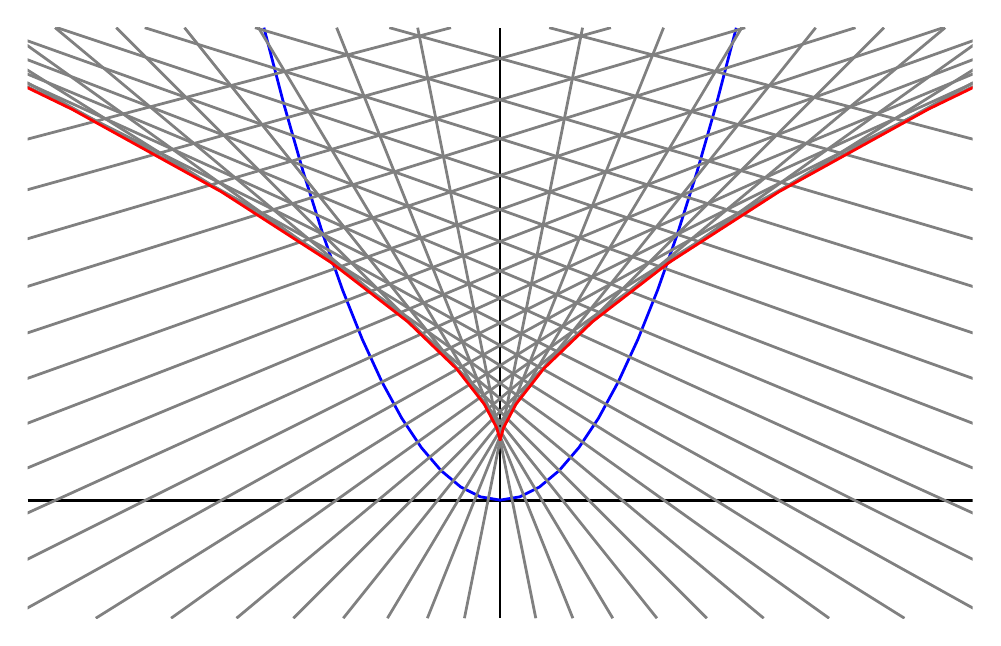
\begin{tikzpicture}[scale=1.5]
%\draw[-Stealth,line width=1pt] (-4,0) -- (4.5,0) node[right] {$x$};
%\draw[-Stealth,line width=1pt] (0,-1) -- (0,4.5) node[above] {$y$};
\clip(-4,-1) rectangle (4,4);
\coordinate (O) at (0,0);
\draw[line width=1pt] (-4,0) -- (4,0);
\draw[line width=1pt] (0,-1) -- (0,4);
\draw[domain=-2:2,color=blue,line width=1pt] plot (\x,{(\x)^2}) ;
\foreach \t in {0.1,0.2,...,1.9}
	\draw[line width=1pt,gray] ({((\t)^2-3.5)*2*(\t)}, 4) -- ({((\t)^2+1.5)*2*(\t)}, -1);
\foreach \t in {-0.1,-0.2,...,-1.9}
	\draw[line width=1pt,gray] ({((\t)^2-3.5)*2*(\t)}, 4) -- ({((\t)^2+1.5)*2*(\t)}, -1);
\draw[red,domain=-2:2,samples=32,line width=1pt] plot ({-4*(\x)^3},{0.5+3*(\x)^2});
%\draw[green,domain=-4:-0.01,samples=32,line width=1pt] plot ({\x},{0.5 + 1.5/2^(1/3)*((\x)^2)^(1/3)});
%\draw[green,domain=0.01:4,samples=32,line width=1pt] plot ({\x},{0.5 + 1.5/2^(1/3)*((\x)^2)^(1/3)});
\end{tikzpicture}
\end{figure*}

解: 抛物线取上一点$(t,t^2)$, 抛物线的切线斜率为 $2t$, 法线斜率为 $-\dfrac{1}{2t}$, 于是法线方程为
\[ y = t^2 + \frac{1}{2} - \frac{x}{2t} \tag{1} \]
所求曲线上的点要满足上述方程, 并且曲线在该点上的切线斜率也是 $-\dfrac{1}{2t}$, 即
\[ \frac{\mathrm{d}y}{\mathrm{d}x} = -\frac{1}{2t} \tag{2} \]
对 (1) 求全微分:
\[ \mathrm{d}y = 2t\ \mathrm{d}t - \frac{\mathrm{d}x}{2t} + \frac{x}{2t^2}\mathrm{d}t \]
然后将 (2) 式代入得:
\[ x = -4t^3 \]
再根据 (1) 可得
\[ y = \frac{1}{2} + 3t^2 \]
这便是所求曲线的参数方程.

~

\noindent 微分方程法

抛物线取上一点$(t,t^2)$, 抛物线的切线斜率为 $2t$, 法线斜率为 $-\dfrac{1}{2t}$, 于是法线方程为
\[ y = t^2 + \frac{1}{2} - \frac{x}{2t} \tag{3} \]
所求曲线上的点要满足上述方程, 并且曲线在该点上的切线斜率也是 $-\dfrac{1}{2t}$, 即
\[ y' = -\frac{1}{2t} \tag{4} \]
利用 (4) 式将 (3) 式中的 $t$ 消去, 可得曲线满足的微分方程:
\[ y = \frac{1}{4(y')^2}+xy'+\frac{1}{2} \tag{5} \]
这是一个 Clairaut's Differential Equation, 对方程两边求 $x$ 的导数:
\[ y' = -\frac{y''}{2y'^3} + y' + xy''\]
再令 $y'=p$, 得
\[ -\frac{p'}{2p^3}+xp' = 0 \]
因为 $p'$ 不恒为 $0$, 两边可以约去 $p'$, 得 $p = (2x)^{-\frac{1}{3}} = y'$, 进而代入 (5) 可得所求曲线方程为
\[ y = \frac{3}{2\sqrt[3]{2}}x^{\frac{2}{3}} +  \frac{1}{2} \]


